\documentclass[a4paper,12pt]{report}
\usepackage{a4wide}
\usepackage{lmodern}
\usepackage[T1]{fontenc}
\usepackage{textcomp} 
\usepackage[utf8]{inputenc}
\usepackage{xcolor}
\usepackage[czech,english]{babel}
\usepackage[pdftex, final]{graphicx}
% \usepackage[pdftex, final, colorlinks=true]{hyperref}
\usepackage{verbatim}
\usepackage{alltt}
\usepackage{paralist}
\usepackage{mdwlist}
\usepackage{subfig}
\usepackage[final]{pdfpages}
\usepackage{amsmath}
%\usepackage[hyphens]{url}
%\PassOptionsToPackage{hyphens}{url}

\usepackage{bibentry}
\makeatletter\let\saved@bibitem\@bibitem\makeatother
\usepackage[final,pdftex,colorlinks=false,breaklinks=true]{hyperref}
\makeatletter\let\@bibitem\saved@bibitem\makeatother
\usepackage[hyphenbreaks]{breakurl}

%%%%%%%%%%%%%%%%%%%%%%%%%
% pro podmineny preklad
% false je defaultně


% \newif\ifbc % Pouze do bakalářské práce
%  \bctrue

%%%%%%%%%% fancy %%%%%%%%%%%
\usepackage{fancyhdr}

\fancyhead[L]{CTU in Prague}

\setlength{\headheight}{16pt}

% \usepackage{stdpage}


%%%%%%%%%%%% rozmery %%%%%%%%%%%%%%%%%%
\usepackage[%
%top=40mm,
%bottom=35mm,
%left=40mm,
%right=30mm
top=40mm,
bottom=35mm,
left=35mm,
right=25mm
]{geometry}


\renewcommand\baselinestretch{1.3}
\parskip=0.8ex plus 0.4ex minus 0.1 ex

\newcommand{\klicslova}[2]{\noindent\textbf{#1: }#2}
\newcommand{\modul}[1]{\emph{#1}}
\author{Štěpán Turek}
% \pagecolor{darkGrey}
\newcommand{\necislovana}[1]{%
\phantomsection
\addcontentsline{toc}{section}{#1}
\section*{#1}

\markboth{\uppercase{#1}}{}
}

\newcommand{\ematr}[1]{
{\bf #1}
}

\newcommand{\evect}[1]{
{\bf #1}
}

\newcommand{\ehvect}[1]{
{\bf \widetilde{#1}}
}

\newcommand{\escal}[1]{
{\it #1}
}

\newcommand{\eucl}[1]{
{\bf R\textsuperscript{#1}}
}
\newcommand{\proj}[1]{
{\bf P\textsuperscript{#1}}
}

\newcommand{\efunc}[1]{
{\it #1}
}


\newcommand{\src}[1]{
{\it #1}
}


%%%%%%%%%%%%%%%%%%%%%%%%%%%%%%
\begin{document}
\pagestyle{empty}

\begin{center}
%napisy
\newcommand{\napisCVUT}{České vysoké učení technické v Praze}
\newcommand{\napisFS}{Fakulta stavební}
\newcommand{\napisObor}{Obor geoinformatika}
\newcommand{\napisKatedra}{Katedra geomatiky}
\newcommand{\napisVedouci}{Ing. Martin Landa PhD.}
\newcommand{\napisAutor}{Štěpán Turek}
\newcommand{\napisDatum}{Praha 2013}
\newcommand{\napisNazevI}{Implementace metody svazkového vyrovnání bloku}
\newcommand{\napisNazevII}{pro určení prvků vnější orientace do programu GRASS GIS}
\newcommand{\napisNazevAjI}{Implementation of bundle block adjustment method}
\newcommand{\napisNazevAjII}{for determination of exterior orientation into GRASS GIS}
\newcommand{\napisBakalarka}{Diplomova práce}
\newcommand{\napisPraha}{Praha 2013}


%
% prikazy
%\newcommand{\velka}[1]{\uppercase{#1}}
\newcommand{\velka}[1]{\textsc{#1}}
%
% 
\newif\ifpatitul
\patitultrue

\ifpatitul
{\Large\velka{\napisCVUT}}\\
\velka{\Large\napisFS}\\
\vfill
{\LARGE\velka{\napisBakalarka}}
\vfill
{\large\napisPraha\hfill\napisAutor}
\newpage
\fi%patitul


{\Large\velka{\napisCVUT}}\\
{\Large\velka{\napisFS}}\\
{\Large\velka{\napisObor}}
\vfill
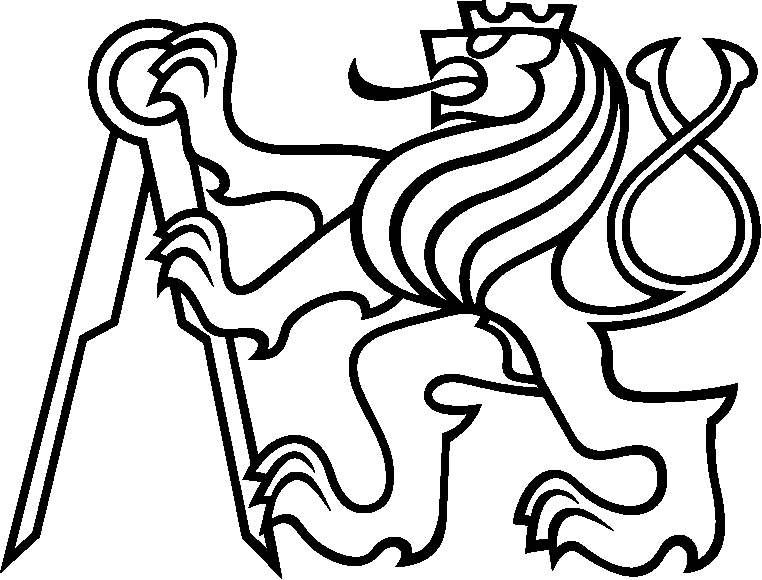
\includegraphics[width=3cm]{logo_cvut_cb} %~
\vfill
{\Large\velka{\napisBakalarka}}\\
{\Large\velka{\napisNazevI\\
\napisNazevII}}\\
{\large\velka{\napisNazevAjI\\
\napisNazevAjII}}
\vfill
{\large%
Vedoucí práce: \napisVedouci\\
\napisKatedra\\
\bigskip
\napisDatum\hfill\napisAutor}
\end{center}

\newpage
\definecolor{navodotisk}{RGB}{10,10,10}
\newcommand{\vlozZadani}{%
\Huge\textcolor{navodotisk}{\textsf{\textbf{ZDE VLOŽIT ORIGINÁLNÍ ZADÁNÍ}}}%
}
%%%\includepdf[picturecommand={\put(100,200){\vlozZadani}}]{zadani}
 % resi si zalomeni sam

\begin{abstract}

\bigskip

\klicslova{Klíčová slova}{GIS, GRASS}

\end{abstract}

\selectlanguage{english}
\begin{abstract}

\bigskip

\klicslova{Keywords}{GIS, GRASS}

\end{abstract}
\selectlanguage{english}


\newpage
\newcommand{\odsaditodzhora}{\hskip1pt\vfill}

\odsaditodzhora
\noindent Declaration of authorship

I declare that the work presented here is, to the best of my knowledge and
belief, original and the result of my own investigations, except as acknowledged.
Formulations and ideas taken from other sources are cited as such.

December 21, 2013

\begin{flushleft}
\begin{tabular}{cp{0.3\textwidth}c}
In Mosty u Jablunkova, 
& 
&
..................................
\\
&&
(author’s signature)
\end{tabular}

\end{flushleft}
\newpage

%%% -> ML: chybi ;-)

\odsaditodzhora
\noindent Poděkování


\newpage

\newpage
\tableofcontents


\newpage
\pagestyle{fancy}

\necislovana{Introdduction}

In recent decades tremndous development of information technology has fundamentally changed many disciplines.

Photogrammetry has sucessfuly taken advantages of this development, and nowadays 
it is using complently different methods and equipment, which allows to obtain and process data 
in huge scales with user friendly methods achieving very good accuracy.

Heavy usage of information technologies likewise caused that borders between disciplines is blurring. 
Photogrammetry was affected by computer vision, which evolved independetly until 2000's. After that it is possible 
to see growing trend of combining knowledge from both fields. 

Both photogrammetry and computer vision are delaing with infomrmation stored in photo. Products of photogrammetry 
are etc. digital elevation models (DEM), which represents earth surface, orthophoto, which is mosaic of merged 
photos thransformed from central projection into orthogonal projection. The orthophoto has same properties.
Nowadays the orthophotos are commonly provided by web ma portals as e. g. mapy.cz or google.maps.com.
The field of computer vision has it's roots in robotics, which is focused on developing robots cabable of 
autonomous behaviour. In order to be the robot autonomous it must know structure of enviroment and its position in it.
This information can be obtained employing methods of computer vision.


The core of photogrammetry is quickly moving  from  hardware towards software. In past it was necessary to have special 
photogrammetric equipment to perform photogrammetric measurement. Nowadays, thanks to current state of the art software, 
 it is possible to use higher level digital cameras to perform photogrammetric measurements achieving
high accuracy. Even with low level cameras, it is possbile to perform photogrammetric measurements. 
Thanks to this shift photogrammetry has not longer been domain of few proffesionals however it is 
becoming used be wide audience. 

We are just at the beggining of the golden age of photogrammetry and computer vision, 
which with spread of UAV and development of augument
reality is going to find a way to our cell phones and other devices we use on daily bases. 

TODO describe difference between ph and cv
Both computer vision and photogrammetry has developed different methods to solve this problem.
The different approaches, how the fields adress the problem, can be generalized to identify 


With growing importance of software there comes a question of licenses. There are two 
main branches proprietary software and free software. Most of proprietary software are not available in 
form of source code. The license of proprietary sofware allows use it under certain terms and usually user 
has to buy it. Proprietary software works like blackbox, because user has no chance investigate the source 
code and realize what his happening. 


\newpage

\chapter{Theoretical part}


\section{GRASS GIS}

\section{UAV}

Unmanned aerial vehicle (also knwn as drone) is aircraft without human pilot. Recently UAVs are known in public by
their heavy military employment in USA and other contries. These military drones are equiped with state of the art 
techonology and their construction is similarly complex as small aircraft.
The number of military UAVs is fastly raising and nowadays USA traines more UAV operators than fighter plane pilots. 
There is also exponentionaly growing sector of civil drones, which is very broad category of various various sizes 
from the big military like size to small devices in size of few decimeters. There are several types of drones e. g. airplanes,
helicopters, multicopters, paraglides, airships, baloons and others. 
Very promising category of drones are multirotor drones (e. g. hexacopters or octocopters), because they have simple construction and 
even ordinary users are able to learn control them very quickly. Together with quickly decreasing prizes of octocopters it can be expected 
that this kind of drone will become commonly used for many civil purposes. 

\section{Least squares}
\label{sec:least}


In linear algebra commonly solved equation is:

\begin{equation}
\label{eq:linear_eq}
\ematr{A}\evect{X} = \evect{L} 
\end{equation} 

which can be interpereted as:
\begin{itemize}
\item \evect{L} - vector of measurements
\item \evect{X} - vector of parameters, which are searched to solve the system
\item \ematr{A} - it is matrix of the cost function  coefitients,  where row represents one measurent 
		  and column represents one parameter of cost function. Linear cost function $\efunc{f_{i}(\evect{X})}$
		  represents relationship between measurements \evect{L} and searched parameters \evect{X}. 
\end{itemize}



If matrix \ematr{A} is 
non singular matrix and vector \evect{b} is non zero vector, then there exists exactly one solution 
for vector of parameters  \evect{X} to satisfy the equation. 

Basically every measurement is burden with some error. The errors can be devided into these main categories:  
\begin{itemize}
\item gross error - error caused by human factor or fault of instrument. If many measurements are repeated
usually it is possble to identify these measurements because they are big outliers from the other measuremnts, which are not affected with this 
kind of error.
\item systematic error - this error has always same effect (value) on measurement.  Usually effect of this error can be 
eliminated by choosing right measuremnt method, calibration of instrument or mathematic elimination.
\item random error - this error is unavoidable becouse it is not possible to know perfectly all factors which has impact 
on the measuremnts. The random errors follows normal distribution which is represented with probability density function of this shape:

TODO picture


The normal distribution is characterized by two parameters, which are standard deviation and  mean. 
If measurements are burden only with random error the mean represents accurate value and standard deviation represents 
dispersion level of measuremnts. 
Theoretically  if measuremnts of some parameter would be repeated infinite times and the measuremtns would be influenced only by random errors,
the accurate value would be computed as  mean of the measuremtns. In case that for measuremt are performed by instruments with different accuracy
 accuraty value would be weighted mean with weight of measurement $\escal{p}_{i}$ defined as:
\begin{equation}
\escal{p}_{i} = \frac{\escal{const}}{\escal{\sigma}_{i}^{2}}
\end{equation} 
where \escal{const} is arbitrary chosen number which is used for calculation of all weights and $\escal{\sigma_{i}}$ is standard deviation of the measuremnt.
It follows that it is possible to get closer to the accurate value by repating of measuremnts, which 
leads into solving overdetermined systems. 

\end{itemize}

The overdetermined systems are solved in many fileds which deals with measurements (e. g. 
surveying, photgrammetry etc.).
As consequence of overdetermination, the matrix \ematr{A} becomes rectangular with more linearly independent rows than  number of columns 
and therefore the solution does not exist for this linear equations system \eqref{eq:linear_eq}.
Only if the measurements would be perfect it would be possible to find such a parameters vector \evect{X}, to 
solve the system of linear equations \eqref{eq:linear_eq}. 

Due to measurements imperfection it is not possible to find such a parameters of vector \evect{X} to make difference \evect{v} between measured values and 
result of cost function using the parameters equal to zero. 

\begin{equation}
\label{eq:least_v}
\evect{v} = \evect{L} - \ematr{A}\evect{X}
\end{equation} 


Hence the least square method finds such a parameters vector \evect{X}, which minimizes 
sum of square differences \evect{v}: 

\begin{equation}
\evect{v}_{T} \evect{v} = min
\end{equation} 


This can be rewritten as:

\begin{equation}
\begin{split}
\evect{v}_{T} \evect{v} &= (\evect{L} - \ematr{A}\ematr{X})_{T} (\evect{L} - \ematr{A}\ematr{X}) \\
&= \evect{L}_{T} \evect{L} - 2 \evect{L}_{T} \ematr{A} \evect{X} + \evect{X}_{T} \ematr{A}_{T} \ematr{A} \evect{X}
\label{eq:least_be_part}
\end{split}
\end{equation} 

The minimum of the function can be obtained using partial derivative of parameters in cost function.
In this case derivatives are simple because it is supposed that our cost functions are linear, thus 
its square forms forms  second degree polynomial e. g. parabola in \eucl{2}, paraboloid in \eucl{3} and all these functions 
regardless dimension has only one point, where the partial derivatives are equal to zero. It is 
their global minimum, which the least squares search for!

The partial derivative of minimized function can be written as:
 
\begin{equation}
\frac{\partial diff}{\partial \evect{X}} = -2\ematr{A}_{T} \evect{L} + -2\ematr{A}_{T}\ematr{A} \evect{X} 
\label{eq:least_part}
\end{equation} 

Giving this equation equal to zero, the global minimum is found:
\begin{equation}
-2\ematr{A}_{T} \evect{L} + -2\ematr{A}_{T}\ematr{A} \evect{X} = 0 
\end{equation} 

The least square is searching for values of parameters vector \evect{X}, which can be expressed from previous equation:
\begin{equation}
\evect{X} = (\ematr{A}_{T} \ematr{A})_{-1} \ematr{A}_{T} \ematr{L}
\end{equation}

This equation is the hearth of the least square method.

The equation suppose that all measurements have same weigh (accuracy). The least squares method can be extended to support weights.
Weight matrix \ematr{P} contains measurements weights on the diagonal with off-diagonal being zero elements in case of assumption that 
the measurements are not correlated.
Row of weight in the matrix determines a measurement in design matrix \ematr{A} where the weight belongs.

The equation, which is minimized by least squares is extended by weigh matrix:
\begin{equation}
\evect{v}_{T}  \ematr{P} \evect{v} = min
\end{equation}

thus the least square equation is altered into this form:
\begin{equation}
\evect{X} = (\ematr{A}_{T} \ematr{P} \ematr{A})_{-1} \ematr{A}_{T} \ematr{P} \ematr{L}
\label{eq:least_sq}
\end{equation}

\subsection{Non-linear least squares}
\label{sec:non_least}
So far it was supposed that cost function is linear and thus global minimum can be found simply by means of linear algebra  \eqref{eq:least_sq}.
Unfortunately in many cases the relationship between parameters and 
measured values is not linear, hence it is needed to adapt linear least squares equations for this case.

Unlike linear least squares, which square of cost function is represented by function  (parabola, paraboloid...) with just one point where all
partial derivatives are being zero, the non-linear cost function can have many such a points (local minimas, stationary points, maximas). 

This problem of non-linearity can be solved by linearization of non-linear equations.
The main idea of linearization is to approximate the cost function with first degree Taylor polynomial,
which is linear and therefore it is possible to use linear least square equation \eqref{eq:least_sq} 
to solve non-linear problem. 

Approximation of cost function with a first degree Taylor polynomial can be written as:
\begin{equation}
\efunc{T^{f_{i}, X_{0}}_{1}} = f_{i}(X_{0}) + \frac{\partial \efunc{f_{i}}}{\partial {X_{0}}} f_{i}'(X_{0}) (X -  X_{0}) 
... \frac{\partial \efunc{f_{i}}}{\partial {X_{0}}} f_{i}'(X_{n}) (X -  X_{0}) 
\end{equation}

where:
\begin{itemize}
\item $\evect{X}_{0}$ is point where the Taylor polynomial touches function, which it approximates. E. g. first degree Taylor polynomial 
      is line, which is tangent of function at point $X_{0}$ in \eucl{2}, in \eucl{3} it is tangent plane and n-dimensional 
      space it is tangent hyperplane.
\item \evect{X} is point where a Taylor polynomial returns approximate value of function $\efunc{f}_{i}$
\end{itemize}


Least squares Taylor polynomial can be written as:

\begin{equation}
\efunc{T^{f_{i}, X_{0}}_{1}} = f_{i}(X_{0}) - a_{0} x_{0} ... a_{n} x_{k} 
\end{equation} 

in matrix form:
\begin{equation}
\efunc{T^{f_{i}, X_{0}}_{1}} = \evect{v} = \evect{L_{X_{0}}} - \ematr{A}\evect{dx}
\end{equation} 

And analogous equation to \label{eq:least_v} can be derived:
\begin{equation}
\evect{v} = \evect{L} - \efunc{T^{f_{i}, X_{0}}_{1}}
\end{equation} 

\begin{equation}
\evect{v} =  \evect{L_{X_{0}}} - \evect{L} - \ematr{A}\evect{dx}
\end{equation} 

and giving:
\begin{equation}
\evect{v} = \evect{l} - \ematr{A}\evect{dx}
\end{equation} 

The accuracy of parameters also determines how many interations (speed of convergence) are needed to achieve optimal solution (global minimum).


and therfore it is possible to use linear least sqaures \eqref{eq:least_sq} for adjustment 
with non-linear cost functions.

However the equation is slightly different. Instead of parameters vector \evect{X} there is used 
parameters vector of differences \evect{dx} and vector \evect{L} is analogous to vector \evect{l}. In this two minor 
substitutions there are hidden major limitations of the non-linear least squares method, 
where prize for approximation is paid. 

As it was already mentioned the Taylor polynomial requires some point $\evect{X_{0}}$.
This approximation is good in close surroundings of point $\evect{X_{0}}$.

Therefore, unlike linear least square method, non-linear least squares requires initial 
value of parameters \evect{X}. If the initial values are not accurate 
enough, it is possible to iteratively run linear least squares subsequently adjusting parameters vector 
to get values, which are in global minimum of the cost function. 

Unfortunately the non-linear least square method has another one more serious pitfall, which 
does not guarantee that it will iterate towards global minimum, where the right solution,
which satisfies minimum squares difference condition,  is situated. If the initial values are 
inaccurate the least squares can iterate toward other local minimas.  
This is caused by run-off of non-linear function, which has more points with zero derivative,
and therefore result depends where the non-linear least square iteration starts.


\subsection{Free network least squares}
\label{sec:free_net_least}

In geodesy usually during least squares adjustment there are some parameters are given as knowns, 
therefore these parameters are not adjusted and network is fixed to this points. 

There must be fixed minimum number of points, which defines coordinate system, otherwise 
matrix \ematr{A} becomes singular. 


In order to be \ematr{A} invertible it is required to fix at least one point in adjustemnt of 1D leveling network.

2D network must have fixed at least two points, because it is needed  
to know two coordinates (shift), rotation angle and its scale for definition of 2D coordinate system. 

3D network requires at least at least 
two points and another point with one coordinate to define coordinate system and thus make matrix \ematr{A}
invertible. The parameters are three coordinates of shift vector, three rotation angles and scale factor. 

Computer vision field uses it for determination of robots position. Very popular is also structure from motion method,
which is able to reconstruct 3D structure from set of images. In essence structure frm motion method is equivalent to the creation 
of digital terrian model.
One of possible methods how to solve this problem is computation of pseudo inverse matrix instead of matrix inversion or 
extend the design matrix with additional constraints.

\section{Short introduction to photogrammetry}

Both photogrammetry and computer vision process set of images, which covers some scene.
The products of processing can be othophoto, DEM, structure from motion etc. 

Essential information which must be obtained or known to obtain all the product is 
interior orientation and exterior orientation of camera.
Exterior and interior orientation together describes relation between object point and
it's corresponding image point.  

\subsection{Interior orientation}

Interior orientation describes relation between measured 2D photo coordinates 
and corresponding 3D in camera coordinate system.

Camera coordinate system has origin in projective point, z axis heading out of the scene  and x, y axes being parallel to photo. 

Photogrammetry equations are based on pinhole camera model, which describes projection of 3D point onto image plane:

Interior orientations parameters describing pinhole camera model are:
\begin{itemize}
  \item Focal length \escal{f} - it is distance of projective center from principal point
  \item Principal point coordinates - In ideal case location of principal point would exactly in the middle 
	of the photo.  
	However in most cases there is some shift of principal point from the photo center.
\end{itemize}

Camera optical system is imperfect, therefore it deviate from the ideal pinhole model  
 causing distortion of photo.

The effect of distortion can be reduced by applying distortion corrections on measured image coordinates. Commonly 
used model for distortion correction is Browns model \cite{brown1966distortion}.
The model defines two types of distortion:
\begin{itemize}
  \item Radial distortion - it depends on distance from principal point. Cause of the distortion is spherical shape of the 
  lens in camera optical system.
  \item Tangential distortion - it is perpendicular to direction of radial distortion. It is caused by 
       imperfect alignment of lenses in camera optical system.
\end{itemize}

Mathematically brown model is written:

\begin{equation}
\label{eq:undistort}
\begin{split}
\escal{x}^{u} =& (x^{ph} - x^{pp})(1 + K_{1}r^2 + K_2r^4 + ...) + \\
&(P_1(r^2 + 2(x^{ph} - x^{pp})^2) + 2P_2(x^{ph} - x^{pp})(y^{m} - y^{pp}))(1 + P_3r^2 + P_4r^4 ...) \\
\escal{y}^{u} =& (y^{ph} - y^{pp})(1 + K_1r^2 + K_2r^4 + ...) + \\
&(P_2(r^2 + 2(y^{ph} - y^{pp})^2) + 2P_1(x^{ph} - x^{pp})(y^{m} - y^{pp}))(1 + P_3r^2 + P_4r^4 ...) \\
r =& \sqrt{(x_{ph} - x^{pp})^2 + (y^{ph} - y^{pp})^2}
\end{split}
\end{equation}
where:
\begin{itemize}
  \item $\escal{x}^{u}$ and $\escal{y}^{u}$  are undistorted coordinates likewise corrected of the principal point shift.
  \item $\escal{x}^{ph}$ and $\escal{y}^{ph}$ are measured photo coordinates.
  \item $\escal{K}_{i}$ are radial distortion coefficients.
  \item $\escal{P}_{i}$ are tangential distortion coefficients.
\end{itemize}


The relation of photo coordinate system and undistorted coordinates is defined as, which is based on the pinhole camera model:

\begin{equation}
\begin{split}
&\escal{x}^{u} = \frac{\escal{X}^{cam}}{\escal{Z}^{cam}} \\
&\escal{y}^{u} = \frac{\escal{Y}^{cam}}{\escal{Z}^{cam}}
\end{split}
\end{equation}
which is clearly visible on this picture:



\subsection{Exterior orientation}

After transformation of 2D photo points into camera coordinate system it is usually necessary to transform it into object coordinate space.
Object space coordinate system must be cartesian. If points are defined in non-cartesian system, it must be transformed into cartesian 
system before using in bellow mentioned equations.

Exterior orientation is defined by position of camera center in object space and orientation of camera coordinate system in the object space .
Photogrammetry uses representation of orientation by euler angles and rotation matrix.

The euler angles are group of three angles, which describes subsequent rotations
 around axes of 3D coordinate system. 
 Order of euler angles is important, because in case of breaching it, resulting orientation is different. 
 In this work there is used notation where at first rotation around y axis is 
 perform, then system is rotated around x axis and the last rotation is perform around z axis.
 
 TODO rotation matrices equation:
 
 
 \begin{equation}
 \begin{split}
\ematr{R} &= \ematr{R}_{z}(\escal{\kappa}) \ematr{R}_{x}(\escal{\omega}) \ematr{R}_{y}(\escal{\phi}) \\
	  &= \begin{pmatrix}
	      cos(\escal{\kappa}) & sin(\escal{\kappa}) & 0 \\
	      -sin(\escal{\kappa}) & cos(\escal{\kappa}) & 0 \\
	      0 & 0 & 1
	      \end{pmatrix}
	      \begin{pmatrix}
	      1 & 0 & 0 \\
	      0 & cos(\escal{\omega}) & sin(\escal{\omega}) \\
	      0 & -sin(\escal{\omega}) & cos(\escal{\omega} 
	      \end{pmatrix}
	      \begin{pmatrix}
	      cos(\escal{\phi}) & 0 & -sin(\escal{\phi}) \\
	      0 & 1 & 0 \\
	      sin(\phi) & 0 & cos(\phi)      
	      \end{pmatrix} \\
	  &=  
	      \small
	      \begin{pmatrix}
	      cos(\escal{\kappa}) cos(\escal{\phi}) + sin(\escal{\kappa}) sin(\escal{\omega}) sin(\escal{\phi}) & 
	      sin(\escal{\kappa}) cos(\escal{\omega})  & 
	      -cos(\escal{\kappa}) sin(\escal{\phi}) + sin(\escal{\kappa}) sin(\escal{\omega}) cos(\escal{\phi}) 
	      \\
	      -sin(\escal{\kappa}) cos(\escal{\phi}) + sin(\escal{\kappa}) sin(\escal{\omega}) sin(\escal{\phi}) & 
	      cos(\escal{\kappa}) cos(\escal{\omega})  & 
	      sin(\escal{\kappa}) sin(\escal{\phi}) + cos(\escal{\kappa}) sin(\escal{\omega}) cos(\escal{\phi}) 
	      \\	      
	      cos(\escal{\omega}) sin(\escal{\phi}) & 
	      -sin(\escal{\omega})  & 
	      cos(\escal{\omega}) cos(\escal{\phi}) 
	      \\		      
	      \end{pmatrix} 
\end{split}
\end{equation}

\subsection{Basic formula of photogrammetry}

Combining of exterior orientation and interior orientaiton it is possbile to define 
direct relation between corresponding 3D point in object space and 2D point
in photo:

\begin{equation}
\label{eq:col_eqs}
\begin{split}
&\escal{x}^{u} = -\escal{f}\frac{\ematr{R}_{11}(\evect{X}^{obj} - \evect{X}^{obj}_{pc}) + 
                                  \ematr{R}_{12}(\evect{Y}^{obj} - \evect{Y}^{obj}_{pc}) + 
                                  \ematr{R}_{13}(\evect{Z}^{obj} - \evect{Z}^{obj}_{pc})                                  
                                  }{
				  \ematr{R}_{31}(\evect{X}^{obj} - \evect{X}^{obj}_{pc}) + 
                                  \ematr{R}_{32}(\evect{Y}^{obj} - \evect{Y}^{obj}_{pc}) + 
                                  \ematr{R}_{33}(\evect{Z}^{obj} - \evect{Z}^{obj}_{pc})     
                                  } \\
&\escal{y}^{u} = -\escal{f}\frac{\ematr{R}_{21}(\evect{X}^{obj} - \evect{X}^{obj}_{pc}) + 
                                  \ematr{R}_{22}(\evect{Y}^{obj} - ) + 
                                  \ematr{R}_{23}(\evect{Z}^{obj} - \evect{Z}^{obj}_{pc})                                  
                                  }{
				  \ematr{R}_{31}(\evect{X}^{obj} - \evect{X}^{obj}_{pc}) + 
                                  \ematr{R}_{32}(\evect{Y}^{obj} - \evect{Y}^{obj}_{pc}) + 
                                  \ematr{R}_{33}(\evect{Z}^{obj} - \evect{Z}^{obj}_{pc})     
                                  }
\end{split}
\end{equation}

These two equations are called collinearity equations, where:
\begin{itemize}
  \item $\escal{x}^{u}$ and $\escal{y}^{u}$ are undistorted coordinates \eqref{eq:undistort}
  \item $\evect{X}^{obj}$, $\evect{Y}^{obj}$, $\evect{Z}^{obj}$ are the point coordinates in object space
  \item $\ematr{R}$ is rotation matrix describing camera system orientation
  \item $\evect{X}^{obj}_{pc}$, $\evect{Y}^{obj}_{pc}$, $\evect{Z}^{obj}_{pc}$ are coordinates of prjection center
  \item \escal{f} is focal length
\end{itemize}

\section{Short introduction into computer vision}

\subsection{Homogeneous coordinates}

In computer vision there are mostly used homogeneous coordinates, which allows to express some relations
mathematically in more elegant way than using cartesian coordinates. 

3D point in homogeneous coordinates is defined as:

\begin{equation}
\ehvect{x} = (\escal{x}, \escal{y}, \escal{z}, \escal{w})
\end{equation}

\escal{w} component is called scale.

The transformation of homogeneous point into cartesian coordinates is done with division 
coordinates by scale:
\begin{equation}
\evect{x} = (\escal{x} / \escal{w}, \escal{y} / \escal{w}, \escal{z} / \escal{w})
\end{equation}

Using homogeneous coordiantes it is possible to write all cartesian points plus points in infinity.
Infinite point in homogeneous coordinates is written as: 

\begin{equation}
\ehvect{x} = (\escal{x}, \escal{y}, \escal{z}, \escal{0})
\end{equation}

Which is impossible to express using cartesion coordiantes with finite numbers:

\begin{equation}
\evect{x} = (\escal{x} / \escal{0}, \escal{y} / \escal{0}, \escal{z} / \escal{0})
\end{equation}

TODO graphic interpretation of hom coords 

Thanks to homogeneous coordinates for planes in \eucl{3} and lines in \eucl{2} it is possible to use simple vector linear algebra operations 
to get useful information.

Plane in \eucl{3} can be written as:

\begin{equation}
\escal{a}\escal{x} + \escal{b}\escal{y} + \escal{c}\escal{z} + \escal{d} = 0
\end{equation}

Using homogeneous coordinates it is possible to express it is as vector:

\begin{equation}
\ehvect{\pi} =  (\escal{a}, \escal{b}, \escal{c}, \escal{d})
\end{equation}


Line in \eucl{2} is defined by equation:
\begin{equation}
\escal{a}\escal{x} + \escal{b}\escal{y} + \escal{c} = 0
\end{equation}

Using homogeneous coordinates it is possible to express it is as vector:

\begin{equation}
\ehvect{l} =  (\escal{a}, \escal{b}, \escal{c})
\end{equation}

It is easy to find out whether point lies on line in \eucl{2}:

\begin{equation}
\ehvect{x}^{T} \ehvect{l} = 0
\end{equation}


Definition of line in \eucl{3} is not so nice as in \eucl{2}.



In homogenous it can be expressed with given points $\ehvect{p}$ and $\ehvect{q}$ as:
\begin{equation}
 \ehvect{l} = \escal{\mu}\ehvect{q} + \escal{\lambda}\ehvect{p}
\end{equation}

If the point is given as direction of the line $\ehvect{d} = (x, y, z, 0)$ (it is infinite point), the equation get simplified:
\begin{equation}
\ehvect{l} = \ehvect{d} + \escal{\lambda}\ehvect{p} \label{eq:hline}
\end{equation}
TODO where not zeros

Simillar equation applies for point on plane in \eucl{3}:

\begin{equation}
\ehvect{\pi}^{T} \ehvect{l} = 0
\end{equation}

Computation of intersection of lines ($\ehvect{l}, \ehvect{l}'$) can be done also in very simple way by cross product:

\begin{equation}
\ehvect{x} = \ehvect{l} \times \ehvect{l}' \label{eq:def_hline_pts}
\end{equation}


Note that with homogeneous coordinates it is possible to express intersection of parallel lines, which lies in infinity, 
therefore it's scale is equal to 0.

TODO dualism

Similarly line can be derived as cross product of two points:

\begin{equation}
\ehvect{l} = \ehvect{x} \times \ehvect{x}'
\end{equation}


\subsection{Basic formula of computer vision}

Computer vision uses this equation to describe relationship between
object space and image space:

\begin{equation}
\begin{pmatrix}
   \escal{x} \\
   \escal{y} \\
   \escal{1} \\
\end{pmatrix}
=
\begin{pmatrix}
   & \escal{f_{x}} & 0     & \escal{c_{x}}\\
   & 0     & \escal{f_{x}} & \escal{c_{x}}\\
   & 0     & 0     & 1\\
\end{pmatrix}
\begin{pmatrix}
   &\ematr{R} & \evect{t}\\
\end{pmatrix}
\begin{pmatrix}
   \escal{X} \\
   \escal{Y} \\
   \escal{Z} \\
   \escal{1} \\
\end{pmatrix}
\end{equation}

In essence this equation is equivalent to collinearity equations \eqref{eq:col_eqs} which are used in photogrammetry.

The equation can be abbreviated as:

\begin{equation}
\escal{w} \ehvect{x} = \ematr{K} \ematr{[}\ematr{R}|\evect{t}\ematr{]} \ehvect{X}
\label{eq:p_exp}
\end{equation}

TODO picture of system

where:

\begin{itemize}
\item \ematr{K} is calibration matrix which contains interior orientation parameters.  
\item \ematr{[\ematr{R}|\evect{t}]} matrix contains rotation and translation, which transforms point from object coordinate system 
	      into camera coordinate system. It is left handed cartesian system, with z axis perpendicular to image plane heading into the scene direction
	      origin in projection center. Difference between camera coordinate 
	      system in computer vision and camera coordinate system in computer vision is the direction 
	      of z axis and thus different handness of system. TODO 
	      Vector $\evect{t}$ can  be transformed in object space coordiantes system:
	      \begin{equation}
	      \ehvect{C} = R_{T}\evect{t}
	      \end{equation}
	      giving coordinates of camera projective center. The parameters \ematr{R} and $\ehvect{C}$
	      represents exterior orientation of camera
	      
\item $\ehvect{X}$ euclidean object space coordinates extended into homogeneous form
\item $\ehvect{x}$ photo space homogeneous coordinates extended into homogeneous form
\end{itemize}

Whole projection can be merged into single matrix \ematr{P}, which is called camera matrix:

\begin{equation}
\escal{w} \ehvect{x} = \ematr{P} \ehvect{X}
\label{eq:p_abbr}
\end{equation}

Camera matrix \ematr{P} defines reprojection up to scale $\escal{\lambda}$, therefore every camera matrix multiplied by scale gives same image points:

\begin{equation}
\ehvect{x}=\lambda\ehvect{P}\ehvect{X}
 \end{equation}

It can be seen as representation of ray going from the projective center. The object point can be located everywhere on this ray, getting always 
same image point coordinates.

\subsection{Two view geometry}

In this chapter there will be introduced theory, which describes mutual relation of two images. 
The core of the theory lies in epipolar geometry.

TODO picture of epipolar geometry
If same object point is identified on two images then there exists epipolar plane.
The epipolar plane contais:

\begin{itemize}
\item two rays which connects object point, with image points and camera centers of both images
\item baseline, which connects projection centers of images
\item epipoles, which are defined as intersection of image planes with baseline
\item epipolar lines, which goes through epipoles and image points. It belongs into image plane, 
      because both these points are inside this plane.  
\end{itemize}


The other relations which comes form epipolar geomatry are:

\begin{itemize}
\item All epipolar lines in image intersects in epipole. If two images are only translated along the baseline 
     the epipole is in infinity.
\item Every image point forms epipolar line in the other image. It allows to reduce space of possible occurrence of the point 
      from \eucl{2}, \eucl{1} of epipolar line, without any other information about the point e. g. object space coordinates. 

\end{itemize}

Algebraic derivation will be done beginning with description of ray in camera coordinate system.
The ray can be defined by two points.
One of them can be projection center $\ehvect{C}$, and 
image point $\ehvect{x}$ transform into camera coordinate system using psedo inverse matrix $\ematr{P}^{+}$, 
where $\ematr{P}\ematr{P}^{+} = \ematr{I}$. After the transformation of x, direciton vector of ray is get.
Using equation \eqref{eq:hline}, it is possible to express ray as:

\begin{equation}
\ematr{X}(\escal{\lambda}) = \ematr{P}^{+}\ehvect{x} + \escal{\lambda}\ehvect{C}
\end{equation}

In second camera with camera matrix \ematr{P'} image point coordinates are:

\begin{equation}
\ehvect{x'} =  \ematr{P'}\ematr{P}\ehvect{x}
\end{equation}

and projective center of first camera is projected into epipole: 

\begin{equation}
\ehvect{e'} =  \ematr{P'}\ehvect{C}
\end{equation}

Having two points in image coordinate system of second camera it is possible to define epipolar line using \eqref{eq:def_hline_pts} as:

\begin{equation}
\ehvect{l'_{e}} =  \ehvect{e'} \times \ehvect{x'} = \ematr{P'}\ehvect{C} \times \ematr{P'}\ematr{P}\ehvect{x}
\end{equation}

Cross product of two vectors \evect{a} and \evect{b} can be also written as multiplication of matrix and vector:

\begin{equation}
\evect{a}  \times \evect{b}  = 
\begin{pmatrix}
   & 0      & \escal{a_{3}}   & \escal{a_{2}}\\
   & \escal{a_{3}}  & 0               & \escal{-a_{1}}\\
   & \escal{-a_{2}} & \escal{a_{1}}   & 0\\
\end{pmatrix}
\evect{b} = [a]_{\times} b
\end{equation}

Using this formulation of cross product it is possible to write:
\begin{equation}
\ehvect{l'_{e}}  = [e']_{\times} \ematr{P'}\ematr{P}\ehvect{x}
\end{equation}

It is evident from this equation, that matrix, which transforms photo points in the first photo into 
epipolar lines of the other photo and thus denoting relation of two images is defined as:

\begin{equation}
\ematr{F}  = [\ehvect{e}']_{\times} \ematr{P'}\ematr{P}
\end{equation}

Matrix \ematr{F} is called fundamental matrix. 

Decomposing fundamental matrix using camera matrix expansion from \eqref{eq:p_abbr} and \eqref{eq:p_abbr}
it is possible to derive another important matrix used computer vision, which is called essential matrix \ematr{E}.

Lets suppose that firs camera matrices are defined in this way:
\begin{equation}
\label{eq:rel_or_cam1}
\ematr{P}  = \ematr{K} \ematr{[}I|0\ematr{]}
\end{equation}
It means that first camera coordinate system lies in the origin of object space and its orientation is same
as axis of the object system.

It's pseudo inverse matrix is:
\begin{equation}
\ematr{P}_{+} =
\begin{pmatrix}
   \ematr{K}^{-1} \\
   \evect{0^{T}} \\
\end{pmatrix}
\end{equation}

And homogeneous projection center coordinates are:
\begin{equation}
\ehvect{C} =
\begin{pmatrix}
   \evect{0} \\
    1 \\
\end{pmatrix}
\end{equation}


The second camera matrix is defined in this way:
\begin{equation}
\label{eq:rel_or_cam2}
\ematr{P}'  = \ematr{K} \ematr{[}\ematr{R}|\evect{t}\ematr{]}
\end{equation}

This relationship of two cameras is also called relative orientation, because rotation matrix \ematr{R} and vector \evect{t}
denotes position and orientation of the second camera to the first one. In order to express cameras exterior orientations in world coordinate 
system or merge it with another relative orientains it is needed to perform further transformations of the relative 
exterior orientations, see \label{sec:ess_chain} and \label{sec:helmert}.

Therefore the fundamental matrix equation can be simplified into:
\begin{equation}
\begin{split}
\ematr{F}  &= [\ematr{P}'\ehvect{C}]_{\times} \ematr{P}'\ematr{P} 
= [\ematr{K}' [\ematr{R}|\evect{t}]
\begin{pmatrix}
   \evect{0} \\
    1 \\
\end{pmatrix}]
_{\times} 
\ematr{K}' [\ematr{R}|\evect{t}]  
\begin{pmatrix}
   \evect{K}^{-1} \\
   \evect{0}^{T} \\
\end{pmatrix} \\
&= [\ematr{K}' \evect{t}]_{\times} \ematr{K}'\ematr{R}\ematr{K}^{-1} 
\end{split}
\end{equation}

Now comes little bit more difficult part:
Using this formula which applies for any non-singular matrix \ematr{K} and vector \evect{t}:
\begin{equation}
[\evect{t}]_{\times} \ematr{K} = \ematr{K}^{-T}[\ematr{K}^{-1}\evect{t}]_{\times}
\end{equation}

the equation gets simplified:
\begin{equation}
\begin{split}
\ematr{F}  &= [\ematr{K}' \evect{t}]_{\times} \ematr{K}' \ematr{R} \ematr{K}^{-1} \\
	   &= \ematr{K}^{-T} [\ematr{K}'_{-1} \ematr{K}' \evect{t}]_{\times} \ematr{R} \ematr{K}^{-1} \\
	   &= \ematr{K}^{-T} [\evect{t}]_{\times} \ematr{R} \ematr{K}^{-1}
\end{split}
\end{equation}

This equation reveals very important fact about fundamental matrix which says that the transformation performed 
by fundamental matrix can be devided into three main steps.
At first photo point of first image is transformed into the first photo camera coordinate system. Result of the transformation is 
point in the infinity, which describes ray represented by image point. 
After that the ray is projected into second camera coordinate system. This is done by so called essential matrix:
\begin{equation}
	 \ematr{E}  = [\evect{t}]_{\times} \ematr{R}
\end{equation}


As the last step, the ray is projected into the second image as epipolar line.


It implies that with known exterior orientation it is possible to define essential matrix. 
Additionally if interior orientation of cameras of both photos are known it is possible to determine fundamental matrix. 
The fundamental and essential matrices are core of two view geometry in computer vision.

\subsubsection{Triangulation of points}
\label{sec:triang}

\subsubsection{Retrieving of exterior orientation from essential matrix}
\label{sec:ess_eo}
Exterior orientation
can be retrivred from essential matrix. However there exists ambiguity of signs which gives 
four possible solutions differing with sings.

The four possible exterior orientation are:

\begin{equation}
[\ematr{R}|\evect{t}],
[\ematr{R}|\evect{-t}],
[\ematr{-R}|\evect{t}],
[\ematr{-R}|\evect{-t}],
\end{equation}

TODO picture

the rotation [\ematr{R}] and vector \evect{-t} can be retrived from SVD decomposition of essential matrix 
where:

\begin{equation}
+- \ematr{R} = \ematr{U}  \ematr{W} \ematr{V}^{T}
+- \evect{t} = \evect{U}_{3,:}
W = 
\end{equation}


Right exterior orientation from four ambiguity can be chosen according simple assumption that all object points has to be in front
of both photo planes (see picture).
TODO


\subsubsection{Merging of relative orientations}
\label{sec:ess_chain}

If two relative orientations are merged together, as first step it is necessary to calculate scale of the two relative orientations.
The scale can be calculated from corresponding distances in both coordinate system. 
It can be used distances of 
object points and object coordinates of projective center of camera, which are present in both relative orientations.

The scale can be computed by this equation:
\begin{equation}
\escal{s}_{ro2-1} = \frac{\mathbf{\evect{X}^{ro1}_{1} - \evect{C^{ro1}_{1}}}}
	                {\mathbf{\evect{X}^{ro2}_{1} - \evect{C^{ro2}_{1}}}}
\end{equation}

where ro1 denotes destination orientation of transformation and ro2 is the transformed relative orientation. 

The equation gets simplified if the relative orientation coordinate system  corresponds to the shared camera system: 
\begin{equation}
\escal{s}^{ro2-1} = \frac{\mathbf(\evect{X}_{ro1})}
	                 {\mathbf(\evect{X}_{ro2})}
\end{equation}

After the scale was determined it is possible to transform exterior orientation in relative system of photo pair into the common relative system.
In order to be transformation easy to express, the common relative system is defined by arbitrary relative orientation of pair and other 
relative orientations are subsequently transformed into this system. 

Set of photos, which can be transformed into common coordinate system, is composed of the relative orientations
which comprise connected component of undirected graph where nodes denotes photos and edges represents relative orientations. 
In other words it is possible to transform relative orientation into the common relative coordinate system only if there 
exist continuous chain of relative orientations where every two neighborhood relative orientations in the chain shares one photo.

TODO PICTURE

The transformation of relative orientations from 1 to n, with common system defined by 1 can be written as: 
\begin{equation}
\label{eq:comm_rel}
\begin{split}
&\ematr{P}_{1} = [\ematr{I}|\evect{O}] \\
&\ematr{P}_{2} = [\ematr{R}^{ro1}|\evect{t}_{ro1}] \\
&\ematr{P}_{3} = [\ematr{R}^{ro1} \ematr{R}^{ro2}| \ematr{R}^{ro1} \evect{t}^{ro2} \escal{s}^{ro2-1}] \\
&\ematr{P}_{n} = [\ematr{R}^{ron} \ematr{R}^{ro(n - 1)}| R^{ro(n - 1)} \evect{t^{ron}} {s}^{ron- (n-1)}] \\
\end{split}
\end{equation}


This equation works for chain of relative orientation, where the shared camera in first relative orientation has 
projection matrix defined by $[\ematr{R}|\evect{t}]$ matrix and the merging second relative orientation is 
defined $[\ematr{I}|\ematr{O}]$. If the camera is defined be the switched coordinate systems, it is needed to 
transform system by multiplication of rotation by $\ematr{R}^[T]$ and shift by $-\ematr{R}^[T]$.

\subsubsection{Helmert transformation}
\label{sec:helmert}

Helmert transgformation equation can be written as:
\begin{equation}
\ematr{X}_{t} = \evect{t} + \escal{s}\ematr{R}\evect{X}] \\
\end{equation}
where \ematr{R} is rotation matrix, \escal{s} is scale scalar and  \evect{t} is translation vector.
The transformation is defined by seven parameters (three translation coordinates, three rotation angles angles and scale).
In order to get these parameters which defines relation of two coordinate system it is needed to know at least two corresponding points and  another one with 
at least one known coordinate in both systems. 



\section{Bundle block adjustment}

Bundle block adjustment is method, which uses the least square technique (\ref{sec:least}) to refine  various scene parameters. 

The main advantage of bundle block adjustment method is that the method is taking into account whole scene and therefore using 
maximum information for adjustment of scene parameters. The principle of BBA has been known for very long time since 1950s.
However the method has been employed in practical application in 1990's, because the performance of computers had not been 
sufficient enough before. 

Cost functions of BBA least squares method are photogrammetric collinearity equations \label{eq:p_abbr}.

Unfortunately collinearity equations are non linear, hence the non-linear least square method \ref{sec:non_least} must be used therefore 
it is needed to provide sufficiently accurate initial values for finding global minimum.

Thanks to the least squares method BBA is very flexible in terms of choosing of parameters to be adjusted. 
It is possible to select various combinations of interior, exterior orientations and object points coordinates parameters 
and refine them using BBA. 


The BBA method is described on practical this practical example.


There are three photos of a scene.
There were identified 3 tie points an 2 ground control points in all three photos.
Other two tie points one ground control point were identified on two photos and one grond control point and one tie point was identified 
on only one photo. 

Let say that initial values of tie points are known, but needed to be adjusted.
Coordinates of ground control points are known with high accuracy, therefore they do not have to be adjusted. 

Every tie point identified on image needs to refine three parameters (object coordinates). 
If the tie point is identified on a photo it yields two measurements (two collinearity equations), 
therefore it is needed to identify the tie point at least on two photos to get more measurements 
than unknowns.

Unlike tie points, ground control point does not bring any new adjusted parameters, therefore
it is possible to use gcp which are identified only in one image. 

In the example we have 3*3 adjusted parameters and 3 * 3 * 2 measurements for every tie point,  
1 * 3 * 3 measurements for every gcp indetified in all three photos. 

We have 2 * 3 adjusted parameters and 2 * 2 * 2 for every tie point,  
1 * 2 * 3 measurements for every gcp visible in two photos.

Tie point identified only in one photo can not be used because number of measurements is smaller (2) than number of adjusted parameters (3).
The ground control point gives two measurements.

Overall score is 15 adjusted parameters and 43 measured parameters.

Thanks to 28 restaurant measurements it is possible to add into adjusted parameters exterior orientation of images (+ 3 * 6) and it is possible to
add some of the interior parameters into adjustment.  

\section{Orthorectification}

Orthorectification is image transformation form perseptive prjection into orthogonal projetion.
Unlike non-orthorectified photo the orthophotos can be merged together into map. Recently 
orthophoto has been widely used by map services like Google Maps or Mapy.cz. Fundamental 
difference of the orthorectified photo and classical photo is that scale in whole orthophoto is same
and therefore it is possible to measure true distances. 


\label{sec:single_ortho}
There are two main methods for producing of orthophoto. The first method is able to produce orthophoto 
from single photo of it's exterior and interior orientations are known and other information which describes
relief must be known. This infromation is usually provided in form of digital terrain model (DTM), which 
can be provided in raster form, which descibes relief whith same density defined by resolution of the raster, 
or vecor surface, which is comprised by continues surface made of trinaglular irregular network (TIN).  
At the beginning of the orthorectificaiton empty raster is allocated, which represents orthophoto, 
which covers photo scene and area of the DTM. After that coordinates are reprojected using collinearity
equations into photo coordiantes. Becouse the DTM surface can be continues, it is needed to define 
same step in which the reprojection is dona. The coordinates can be choosen e. g. from ever pixel center
of the orthophoto pixel. Results of reprojection are not pixels cordinates which is integer number but 
floating points numbers. Therfore value of pixel in orthophoto can be computed by different interpolation methods,
which can take various number of neighbourhood pixels and functions.

The other method is being used either in computer vision and photorammetry. In computer vision 
it is called structure from motion. As the method name suggests, it is primarly used for retrieving
strucure of the scene, which is equivalent of DTM in photogrammetry. In follows main advantage 
of the mathod that DTM does not be needed unlike the first method DTM is not needed. Moreover 
the DTM can be another result besides the orthophoto if this method. The method is based 
on forward resection, where collinearity equations are employed. The other approach requires to have at least
two photos of known exterior and interior orientation. In contrast to the first method the exterior orientaiton
can be defined in arbitrary coordinate system, because there is not needed to define relationship to 
known DTM, therfore it is possble to generate orthophoto and DTM without need to have GCP. However 
if the results should be transformed into world coordiante system it least three GCP needs to be known
to perform Helmert transformation. 

The principle of the method is based of forward ray intersection. In order to find object coordiantes
of point, the point has to be identified at least on two photos, than two rays connecting projection 
center and image points are formed. The approximate object coordiantes can be find by trianglulation 
method \ref{sec:triang} and than refined by BBA, which is also in principle based on the rays 
resection.
 

\chapter{Analytical part}

In this part there are describe reasons, which led into development of process chain which was implemented in 
this thesis. All methods of the processing chain which are mentioned in this chapter, where described in 
previous theoretical chapter.

\section{General solution of UAV bundle block adjustment}


Few years ago in late 1990s it seemed that prolem of approximate values for BBA had been solved. 
In this times BBA was mainly employed in aerial photogrammetry. Mapping mission using aerial 
photogrammetry are done by experts and budget of such a mapping missions is very high. 
The development of GPS and IMU uints, which allows to determine 
postion respectively and orientation with propelly set up and calibrated camera and GPS/IMU 
units allowed to get very precise approximate values of exterior orientation, therefore 
it was possible to use it directly in BBA.

  
As it was already mentioned the development of technology gives oportunity to many poeple
to perform photogrammetric measurements, because nearly everybody has camera in his pocket.
On the other hand the solution must be very simple from the user point of view becouse 
most of users has limited or no knowldge of photogrammetry. It follows the main requirement 
on solution, which was set up at the beginning of the thesis.

To make this requiremement of simplicity more specific the user should be able to used it having 
just camera and UAV. No other hardware device should be needed. All other steps should be done 
using open source software which can everybody download.

Also the solution should be flexible enough to process aditional data, which may known, 
as GCPs approximate postion of cameras etc.With this aditional data it is possible 
to increase accuracy of results and decrease number of  BBA iterations needed for finding 
global minimum. Therfore it could be used by more advanced users.

As consequance of these contraints, the minumum input into processing chain can be just photos
of the scene and other parameters, which can be derived from information on specific kind of photos.

The another important requiremnt is two make the process as much automatic as possbile, because 
if it would require a lot of time of user to go through the processing chain nobody would use it.

To fulfil these requiremnts the solution can be described by this prcessing chain:

\begin{itemize}
\item Camera calibration - getting interior orientaion of camera.
\item Relative orienations of photo pairs - getting interior orientaion of camera.
\item Triangulation of tie points - getting interior orientaion of camera.

\end{itemize}




\subsection{Camera calibration}
\begin{itemize}
\item Camera calibration - during camera calibration processs, the interior orientation parameters 
			   are determined.
		             Interior orientaiton can be computed 
			     from multiple photos of 2D or 3D test fields. As the test field it can be used 
			     paper with printed pattern, which can everybody do. 
				
\item Obtaining approximate exterior orienation parameters - solution should work also with photos 
which does not have known exterior orienation paametrs at all. It means 
that GPS and IMU unit does not have to be mounted on UAV and calibrated with camera.
  

\item Refine the scene parameters using BBA - As input to the BBA aproximate obtainded exterior orientation
and interior orientation from camera calibration are used.

\end{itemize}

If only information which is available about the scene is interior orientaiton parameters and the photos, 
only way how to obtain aproximate exterior orientation of cameras and recover the scene structure is 
by identification of some tie points in the photos. If the scene is taken from one image, there is no way how
to retrive exterior orientation of camera if no additional information about scene e. g. gcp is not known. 
The same thing applies for photos taken with  unsufficient overlap because it is not possible to 
identify enough tie points. The last constraint is that the photos can not be taken from same position.

\subsection{Tie points identification}

The simpleist way from developer point of view is to force user to indentify tie points on 
the photographs manually. However users would have to waste a lot of time on such a 
dull task. Fortunatelly there  exist algorithms, which are able to identify tie points on images
automatically. The state of the art algorithms are SIFT \cite{wiki:SIFT} and SURF \cite{wiki:SURF}.
These algorithms allows to indentify tie points on photos, whithout need to include any other information.
Unfortunatelly both algorithms are patented in USA, therfore they use should be avoided open source community.

Recently new BRISK \cite{leutenegger2011brisk} and FREAK \cite{alahi2012freak} algorithmd 
has been developed, which does not have patent restriction. 

Another problem of tie points matching is determination of photos order, to identify photos with some overlap. 
If photos are taken in strip, it is easy to deal only with neighbour photos to identify the tie points.

If there is no apriori information about image order, the easiest way is to use brute force and 
try to find tie points in all images in set. With higher number images this problem become 
hard to compute in resonable time. To avoid this it is possbile to build up visibility map \cite{barazzetti2010extraction}, 
which is graph with photos as nodes. The graph edges connects photos and represents existing scene overlap 
in photos. For creation of visibility map it is possble to use information from GPS and IMU units.

Another speed up can be done decreasing resolution of images 
for first search of tie points. This first search should only identify connected images.
In second step tie points etraction is done on full resolution but only in imges which 
are connected .

This part was covered in this thesis just with this short overview, becouse this topic is so big 
that it would be possible to write masters thesis focused only on feature extraction or building 
of visibility map.


\subsection{Retrieving approximate values for bundle block adjusmtent}


The next step is to utilize all known information (interior orientaitn and extracted 
tie points image coordinates)  to get missing approximate parameters for BBA. 

Because collinearity equations \ref{eq:col_eqs} are the cost functions in BBA ,
extracted image coordinates represents measurement (result of collinearity eqation),
the parameters of interior orienation are known from the imput and only information 
which is misisng are aproximate parameters of exterior orientation and object coordinates of 
tie points. 

\subsubsection{Aproximate values of exterior orienation}

There exist many methods how to obtain approximate values for exterior orientaiton of cameras, they 
differs in information which they require for input, computation time and accuracy. 
To fullfil the set up requirements the chosen method should be able to retrieve exterior orientation 
using image coordinates of tie points and interior orientation of camera.
Also it should be used some method for determination of 3D coordinates of the tie poitns.

There exists lot of methos which are able to retrie EO using aditional 
information about scene and the EO of camera.

In aerial photogrammetry is is possible to suppose that photos are nearly verical and therfore 
rotation matrix can be simplified resulting in 

Furtunately there exists family of closed form computer vision algorithms,
which are able to determine relative orientation (essential matrix) from image coordinates 
of the tie points. The algorithms are based on epipolar geometry using essential matrix 
constraints to find the solution. 

The closed form algorithms are called accoridg to required number of identified tie points in two pictures.
There exist eight, seven, six and five point algorithms. The five point algorithm seems to perform best in most
of cases \cite{stewenius2006recent} and it is not sensitive on planar points configuration.

Only case when the five point algorithm \cite{nister2004efficient} underperforms 
\cite{bruckner2008experimental} the others is forward motion of camera.
However this should occure in very rery cases  if UAV is used for mapping.

Main disadvantage of the five point algorithm is that it can produce up to ten solution.
Therfore it is needed to select best solution from these. The number of solutions can
can be reduced by testing assumption that the tie points should lie in fron of the image 
planes of both cameras. After sorting out obviously non sense solution in previous step
 the optimal solution can be chosen the one which has minimum sum of tie point distances
 from epipolar lines, which were computed by corresponding tie points in the other photo
 using essential matrix of the solution and calibration matrix of the photos cameras.  

Because matching algortihms are not perfect  certain number of the tie points are matched 
incorrectly threfore it is needed to be the relative orientation method robust enough to
deal with these outliers.

The RANSAC \cite{RANSAC} method is comonly used with this family of epipolar algorithms to 
make it robust for effect of outliers.

Principle of RANSAC is to find such  a solution in group of measurements with outliers, 
which well aproximates the inliers. 

In case of the epipolar family algorithms RANSAC works that in every iteration 
in selecets random tie points, which used epipolar algorithm requires and 
runs this agorithm. After obtaining an essential matrix from the algorithm the epipolar 
distances for tie points are computed. There is specified some threshold of the distance which is used 
for decision whether the measurement is inlier or outlier. The other threshold, which has to be specified 
is percentage of inliers of all tested points. If percentage of inliers is highest than in prevous iteration,
the essentail matrix is set as the best fitting and iteration continues. The iteration terminates after user defined 
number of iterations with returning the best fitting essential matrix.

\subsection{Aproximate values  of tie points object coordinates}

After essential matrix is obtained it is possible to compute object coordinates of tie points with trinanglutation
method.

The triangultation can be done by several methods. If the measuremtns would be precise, the 3D point 
would lie in intersection of two rays wich are lines conecting projection centers and image points 
in the photos. Unfortunatelly the rays are never determined so precisly, thus it is needed to deal 
somehow with the errors. 

To solve this problem it is possible to use linear least squae methods. The solution is based 
on direct linear method, which is linearized form of collinearity equation \eqref{eq:col_eqs}.
\begin{equation}
\label{eq:col_eqs}
\begin{split}
&\escal{x}^{im} = \frac{\escal{a}_{1}(\evect{X}^{obj}) + 
                                  \escal{a}_{2}(\evect{Y}^{obj}) + 
                                  \escal{a}_{3}(\evect{Z}^{obj}) +
                                  \escal{a}_{4}
                                  }{
				  \escal{a}_{9}(\evect{X}^{obj}) + 
                                  \escal{a}_{10}(\evect{Y}^{obj}) + 
                                  \escal{a}_{11}(\evect{Z}^{obj}) +
                                   1  
                                  } \\
&\escal{y}^{im} = \frac{\escal{a}_{5}(\evect{X}^{obj}) + 
                                  \escal{a}_{6}(\evect{Y}^{obj}) + 
                                  \escal{a}_{7}(\evect{Z}^{obj}) +                                 
                                  \escal{a}_{8}
                                  }{
				  \escal{a}_{9}(\evect{X}^{obj}) + 
                                  \escal{a}_{10}(\evect{Y}^{obj}) + 
                                  \escal{a}_{11}(\evect{Z}^{obj}) +    
                                  1
                                  }
\end{split}
\end{equation}

This method is easy to implement and there is no need to know approximate vaules.


Main drawback of this method is that DLT model is not based on true projective geometry, thus 
if elements of \evect{a} would be takend as unknowns in adjustment, the computed corrections 
would not respect the projective transformation constraints.  In trinanglutation of image points 
it is supposed that vector \evect{a} is known. However the vector \evect{a} is never determined 
totally preciselly and therfore found solution does not have to be optimal.
TODO

The more complicated method from computer vision is called the optimal solution. 
It is based on enforcing epipolar constraint, whith cost function 
minimizing distance of projected points from the other images to epipolar lines.

The cost function is not linear however it's derivative leads into 6 degree polynomial thus 
having 6 roots.

This method is seen by computer vision community is most accurate \cite[p. 315]{Hartley2004}.  


\subsection{Common relative coordinate system}

Currently all approximate values which are needed in \eqref{eq:col_eqs} are available for BBA. 
The problem is that it is not possible to adjust scene in one bundle, because tie points
object coordinates and exterior orientaions are all related to the two photos, which they were 
retrieved from. The two views defines it's own relative object coordinate system which is identical
to the first camera coordinate system \eqref{eq:rel_or_cam1} and
exterior orientaion in the system of the second camera \eqref{eq:rel_or_cam2}.


Therefore it is needed to transform all features in the two view coordinates systems into 
an common coordinate system. First of all the common system has to be defined.
In order to make the transformation process simple it is defined by one of the two view
systems.

The next step is to connect successively the two view systems into the common one.  
An block of the two views systems, which can be merged, is composed of the systems 
where exists path from the pair which defines common system.

The path exists if there is chain of neighbourign two veiw systems, which 
shares one photo. 

Another problem is that the two view systems are defined up to scale therefore 
it is needed to determine scale of merged system related to the common one. 
The scale can be computed by comparison of distances which are common in both systems.
One approach is to use tie points object coordinates in both systems 
and compute distances from projection center which belongs to the shared photo \ref{seq:ess_chain}. 


\subsection{Transformation into world coodinate system}

Usually the user wants to be measurement transformed into an world coordinate system, which allows 
to compare measuremtns with other data, which are available in this system or they are 
linkend with the world system which is usually connected to all other commonly used  world systems. 
This transformation is called Helmert  transformation and it can be basically devided into 
three main steps which are rotation, scaling and translation \ref{seq:helmert}.

In order to be transformation of the common system into the world system be possible, it is needed 
to have at least 3 tie points, with known approximete coordinates in the common space, which also have 
known coordinates in the world system. These points are called ground control points (GCP). The other advantage is that it is possible to use GCPs for improving accuracy of the results and 
 quality assesment of obtained results.
 
This step is optional, it is possible to perform bundle block adjustment in the common system. In this 
case it is needed to perform BBA of free network \label{sec:free_net_least}. 
 
 
\subsection{Bundle block adjusmnet}

So far all aproximate values of parameters in collinear equations are obtained therfore it 
is is possible to perform the bundle block adjustemnt, which finds the optimal solution.

In essence there exists two main types of the adjustment, which can be used. The scene 
can be adjusted as free network if there are known less that 3 GCPs or it is possible 
to use information about gcp and use non-linear least square method.

\section{GRASS GIS Orthorectification Workflow}

GRASS GIS supports is among few open source GIS software which supports orhorectification ed
\cite{rocchini2012robust}. Orthorectificaion is done by 
by i.ortho.photo \cite{i.ortho.photo}, which was developed 1990s.
I.ortho.photo is specialized on processing analog aerial imagery, therfore 
it supports to transformation of scanned photo using fiducial marks. 
The interior orientation parametrs are supposed to be known without taking distortion 
coefitients into account. 

The next step of is retrieving of exterior orientation parametrs. The retrieving 
of exterior orienation is based of least square iteration. Unlike BBA
the photos are adjusted separately, therfore the object points coordinates has to be known
and there has to be at least three ground control points becouse six exterior parameters are 
searched. The three gcps are just theoretical minimum, however for getting resonable 
results it is needed to provide at least 12 parameters. Exterior orientaion 
can be attached into input to be used as approximate values for iteration,
otherwise it is supposed that images are verical, therefore two of three rotaion
angles can be set to 0 and the last angle is computed as difference of centroid slope
in photo system and object system taking into account only x, y coordinates.
Projection center object coordinates are given equall to centroid coordinates.

In the last step the orthorectified image is computed. GRASS GIS uses single image orthotectification
method \label{sec:single_ortho}, which requires known DTM in order to deal with height differences. 


The main disatvage of GRASS GIS orthorectification method are:
\begin{itemize}
\item Orhorectifies photos separately, thus it ignores significant part of information unlike BBA,
 which can improve accuracy and robustness of orthophoto. 
\item Because of single photo orthorectification method it is neccessary to have DTM of scene to 
generate orthophoto. Priecise high resolutin DTM is not usually available for free so this 
requiremnt should be avoided.
\item If exterior orinentation of the camera is not known, implemented method for exterior
orientaiton retrieving needs GCP, which may not be always available. Moreover  if the images 
are not vertical, it is needed to know at least approximate exterior orietnation valuas for 
convergence towards global minimum.
\end{itemize}

These disadvantages are big obstacle which make difficult to use current implementation of GRASS GIS 
to process UAV acquired photos, which often lack GCP and DTM information.
On the other hand the current GRASS GIS orthorectificaiton method can be succesfully used  
if all required information is provided.

\chapter{Implementation}

\section{Used technologies}

\subsection{OpenCV}

OpenCV is open source computer vision and machine learning library released under BSD licence. 
The library contatins thouasans of algorithms, which are mainly focused real time image processing.


The OpenCV library contains also algorithms which can determine eterior orientaiton and object coordinates 
of the tie points which ca. 
Another relevant group of algorithms deals with camera calibration. Using the agorithms

\subsection{Python}

Python is open source programming language which has been developed since 1991. 
The python code has is easly readable and therefore it is often picked as first programming
language to learn. Python is empoyed in wide range software from simple scripts to complex systems.
It is higher level programming language comapared to languages e. g. C++, therefore 
the development process is usually significantly faster. On the other hand 
to Python is significantly (hundred times) slower compared to C+. Even so big 
slow down does not have to be reason for avoiding Python in development. 
In many application the Python is used as top level glue, which took care about 
tha main workflow. The parts of aplication, which do heavy computation  they can 
be written in other mote efficient algorithms and then being called 
from Python. This is very powerful combination, which allows to speed up development 
process preserving speed of application.

Thanks to the its popularity the Python world is very rich. There are developed
thousands of open source libraries, which make life of programmer much of easier. Even 
if library is not implemented in Python it is possible to generate Pythonic 
interface using some of available open source tool (e. g. SWIG), which automaticaly
generates the interface. And even if the library does not have Python interface it 
is possble to use the tools as e. g. ctypes or Cython to use libraries directly.


\subsubsection{NumPy}

NumPy is open source Python library, which supports multidimensional arrays and many operations, which can be
performed using this arrays including linear algebra operations. Killer feature of NumPy is its speed,
which allows to write very effective code with just few lines. Many operations which NumPy do can be 
also rewritten be Python code using  for loops. However if numpy function is called,
computation is perform by very quick C code, which can makes big difference if arrays contain 
lot of elements. Sometimes it is difficult to figure out the way how 
to write problem using Numpy avoiding fot loops  for beginner. However as a user gets experienced 
it become easy to do it. 

NumPy is so widely used Python library that it has become one of fundamental libraries, thus many
other libraries has already integrated NumPy support ore they require NumPy installation.

\subsubsection{SimPy}

Simpy is another python library which is focused on process-based discrete-event simulation.
Among many other features it supports symbolic expression. This symbolic expression can be useful
e. g. for computation of derivation of an function. The result of dervation is symbolic expression which can 
be than used for retrieving numeric values. 

\subsection{GRASS Programming  enviroment}

The recommended languages for development of GRASS GIS modules are C and Python.




\section{Implementaiton into GRASS GIS orthorectificaiton workflow}

The implementaiton should fulfill these goals:

\begin{itemize}
\item Backward compatibility, which preserves already implemented functionality, which
can be still useful in specific cases. 
\item Take advantage of modularity of i.ortho.photo module.
If the workflow is comprised of modules with clearly defined interface, it is possible to implement
several different algorithms for every step of orthorectificaion. The main advantage is this 
aproach is that workflow can be adapted to the specific situation, which allows to use 
most suitable algorithms to achive maximum accuracy.
\item For the less advanced users, which does not have suffucuient knowledge to create individual 
worflow there should be another module, which is easy to use, and wraps the more specific mudules.
Eventually graphical user inteface which helps with assesment of developed data and running orthoectification
should be developed. 
\end{itemize}

If all this goals would be fullfiled GRASS GIS would become unique flexible state of the art orthorectificaion 
software, which could be used by wide spectrum of users from amateurs to experts.
Due to time limitation this thesis deals only with lowest level modules, however it is very important to have 
the ultimate goal in mind to desing solution from basis properly in order to save a time in future spend 
on refactoring.

In order to meet the implementaiton requirements these main steps can be implemented in form 
of these GRASS low level modules:

\begin{itemize}
\item Camera calibration modules - Retrieves interior orienation, which is supposed to be known by 
next steps of the workflow, therfore this step can be represented be the calibraiton module.
\item Point match modules - Identification of tie points in the acquired images, which is out of the 
scope of the thesis.
\item Intial values modules - This module computes intial value of extrior oritnetation and 
object coordinates of tie points, which are used in BBA. It uses information from the both
previousle mentioned module.
\item BBA modules - The module perform BBA based of date obtained be the other modules.
\end{itemize}


\subsection{Camera calibration module}

The calibration module i.ortho.cam.calibrate is simple module written in Python, which calls
function from OpenCV calib3d module. The module is based on calibration from 2D patern, which can 
be easily printed. Most important imput parameter defines directory with images of 2D pattern, 
taken by the camare. In order to obtain good results of camera calibraion, at least 10 images 
from different positions all around the pattern should be taken \cite{camera_calibration2013opencv}.

Currently OpenCV supports these three patterns:
\begin{itemize}
\item Chessboard pattern 
\item Asymetric pattern of circles
\item Symetric pattern of circles
\end{itemize}

Generally the circle patterns achieves higher accuracy \cite{camera_calibration2013opencv}.

The identificaiton of pattern points (centers of circles or corners of chessboard squares) 
are done by OpenCV functions, which are able to identify the points on photo of the pattern 
without any other additional information except numpber of circles or squares per row and column
of the pattern. Then the points coordinates in the photo are refined to subpixel accuracy.

Photo coordinates identified in the pattern photos together with object coordinates which can be chosen
arbitrary according to pattern type and number of rows and columns of pattern marks. 
No other information is needed to retrieve interior orinentation of camere. The method is described 
in \cite{zhang2000flexible}.

The computed interior orinetaion is saved into GRASS GIS camera file, which is used by other GRASS GIS 
orthorectificaiton modules. The module modifies the camera file via i.ortho.camre module.
The GRASS GIS camera data model was extended to support radial and tangetial distortion coeffitients, which 
have serious effect especially in cheap cameras, where optic system is not so precise.

\subsection{Bundle block adjustment data model}
 
Both the intial values and BBA modules basically handles  same data, thus 
the data model can be designed in similar way. There can be 
identified three essential classes, which are shared by both modules :
\begin{itemize}
\item Camera - the camera class has to store information about interior orienation 
parameters including distortion. Camera class should contain referecnes of the photos
clasess, which were acquired with the camera.
\item Photo - members of photo class are references to the points, which were identified 
	    in the photo and camera with the photo was taken,
\item Point - the poitn object denotes representation of same object point in different images (tie points).
 If the point is GCP it includes also information about it's object coordinates. 
\end{itemize}


This classes offer enough flexibility for both modules adaptation, which can be done be done by subclassing. 
Likewise it sufficiently expresses  structure of the data and relations of the data structure elements.

\subsection{Initial values module - i.ortho.initial}

The i.ortho.initial module retrieves intial values of exterior orientation of the cameras and inital tie points object coordinates. If at least 3 gcps are 
present in an input, relative coordinate system is transformed into world coordinate system of the gcp by applying Helmert transformaiton. 


The module needs for input these 
\begin{itemize}
\item Interior orientations of cameras e. g. computed by i.cam.calibrate
\item Tie points photo coordinates 
\end{itemize}

The module first builds interally graph like structure, where nodes represents images and edges holds information 
about number of corresponding tie points, which are identified on two photos which edge links together.
Than the relative orientaion of photo pairs is performed. The photos are oriented by going through the graph. 
The the pair of photos which are taken for the relative orienation are the photos with the highest number of the corresponding tie points. 
The next candidate is chosen from the subset of neighbourhood photos, which have not been already relativly oriented. The chosen pair 
must also satisfy the highest number of corresponding tie points in the pair. Tha pair is comprised of one photo is already 
part in at least one relative orietnation and the second photo is newly oriented. The relative orientaion of the photo 
pair is performed by  the five point algorithm, which has been recently added into OpenCV as function findEssentialMat \cite{calib_manual2013opencv},
which returns the essential matrix. Exterior orientaion is retrieved \ref{ess_eo} from the essential matrix by Rodrigues \cite{calib_manual2013opencv} 
function. Because the exterior orientaiton is defined by relative coordinate system of the two cameras, it is needed to be transformed into 
the common relatrive coordinate system. The coomon system is defined by the relative orientaiton coordinate system of the first pair.
Every other relative system orientaito is connected to the common system by the chaining of essential matrices see \label{sec:ess_chain}.
The last optional step of the module is transformaiton of the relative coordinate system into the word coordinate system. The helmert 
transformation is performed by code from \cite{v.rectify}, V.rectify module is uses e. g. for transformaiton of Lidar point clouds 
into world coordinate system. Besides other transformation it supports also helmert transformaiton. The code, which computes Helmert 
transformation \ref{sec:helmert}, was moved from the v.rectify module into the GRASS GIS imagery library in order to be accesible also  by i.ortho.initial
module. The known helmert transformaiton cooffintients are applied on the exterior orientaitons of cameras and objecet coordinates of the tie points.

The output of the module are exterior orientations and object coordinates in comon relative or world coordinate system. Together with interior
orientation parameters and image coordinates all needed information is obtained  for the i.ortho.bba module which performs final bundle block adjusmtent 
iteration.  

\subsection{Bundle block adjustment module - i.bba}

The bundle block adjustment module perfroms non-linear least squares iteraion for collineariry equations. 
The input into module represents all parameters of collinearity equaitons:
\begin{itemize}
\item Tie points photo coordinates e. g. identified manually or be automatic points matching algoritmhs
\item Interior orientations of cameras e. g. computed by i.cam.calibrate
\item Exterior orientations of cameras e. g. approximate values can computed by i.ortho.initial
\item Tie points object photo coordinates e. g. identified manually or be automatic points matching algoritmhs
\end{itemize}

The module performs linear non-least square iteraiton until correciton of the parameters from the adjusmtent are smaller than
defined treshold. The module supports is able to perform non-lineart least squares as free network or using selcted points 
as knowns (at least three) and thus solve in classical way.
TODO parameters adjustment definition


The output of the module is the adjusmtent protocol which is attached in the Appendix \cite{sec:adj_protocol}. In the protocol, there
is described every iteraiton of the bba including correction for all adjusted paramaters and standard deviaitons computed from 
covarinace matrix of the adjustment. 




\chapter{Test case}

The processing chain was developed and tested on data, which were kindly provided by Martin Rehak. The available 
information about scene included:

\begin{itemize}
\item Tie points identified on the photos
\item Position of cameras (leverage arm offset + gps coordinates)
\item GCPS
\item interior orientation of camera, which acquired the photos of the scene
\end{itemize}


Also there was included protocol of BBA from Bingo-F software \cite{bingo2013gip}, which reveals 
the processing steps, which the software uses.
In general information form this protocol was very helpful for me, because 
 it should me how the processing chain should look like.

Bingo-F is widely used well tested software software, which is used by many users on various  scenes configurations.  
Compared to the developed processing chain in this thesis it is miles ahead, therefore the results of the Bingo-F adjustment were 
regarded as reference for obtained data from the developed processing chain.

Generally Bingo-F processing is very similar to the developed  processing chain of the developed solution, which is  
described in-depth in previous chapter. First step is the relative orientations of pairs, then the pairs are merged into common relative 
coordinates system. After that helmert transformation is performed into world coordinate system and as a last step BBA is performed.

Unlike the developed processing chain,  the Bingo-F software was taking into account also information about position of cameras during the adjustment. 
Because the developed processing chain should be general as much as possible it was decided that in first version  the processing chain would ignore this 
information because according the aims set up in the previous chapter the final solution should require tie points photo coordinates and interior 
orientation of cameras. Anyway later it is possible to extend the processing chain to work also with such additional information to improve accuracy 
of the results. 

Also the Bingo-F is capable to identify and rule out blunders in every step of processing chain and thus it is more robust. 
In final BBA it computes weights probably according to defined standard deviations of parameters, which are available in the data. Also computation 
of BBA is optimized therefore it is possible to solve scenes with thousands of tie points.

Output  protocols of Bingo-F adjustment contains: 

\begin{itemize}
\item Interior and Exterior orientations of photos
\item Object coordinates of tie points and gcps
\end{itemize}

The scene was adjusted as free network, adjusting interior orientation parameters (focal length, principal point coordinates),
exterior orientations of photos, and object coordinates of all points. It was also adjusted lever-arm offset which describes 
shift of GPS unit from projection center.  Lever-arm offset allows Bingo-F to use information of photo positions from GPS unit,
which is shifted by this offset.  

Final reconstructed  scene from Bingo-F results is shown in this plot:
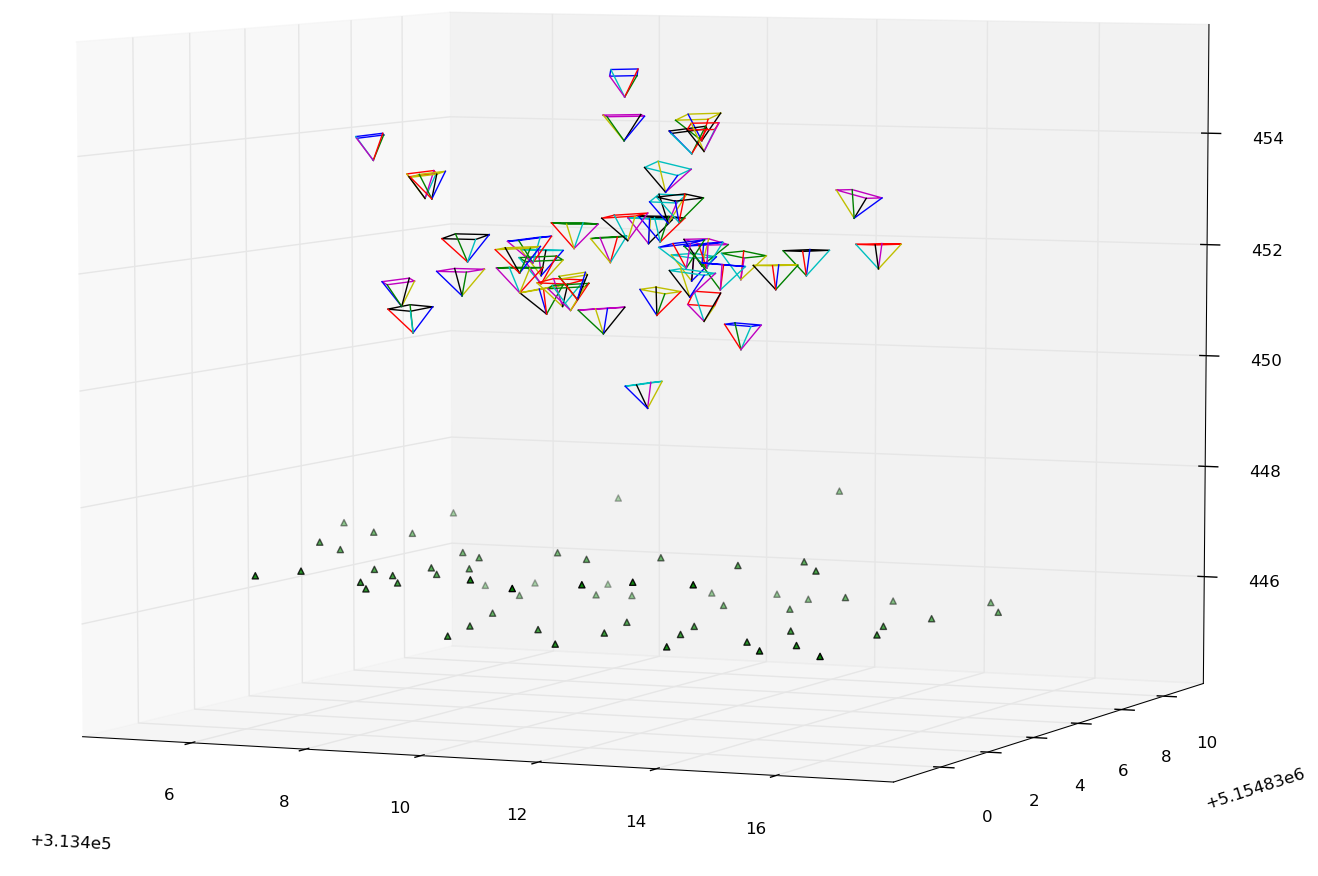
\includegraphics[scale=0.5]{figures/bingo_result.png}
Unlike many other real scenes which can be comprised by hundreds of photos and thousands of tie points,   
there are just a few tie points (64) and photos (45) taken by same camera. Also the photos capture same points thus there 
is lot of redundancy, which should improve robustness of the bba. 

In the rest of the chapter there will be presented results of subsequent steps, which are performed in processing chain and compared 
to the Bingo-F results.

The first step is relative orientation of pairs. The relative orientations of the pairs were done by OpenCV 5 point algorithm.
The algorithm was successful on most of the pairs, however there are some pairs were algorithm does not work well.

Example of the algorithm success can be showed in this plot:
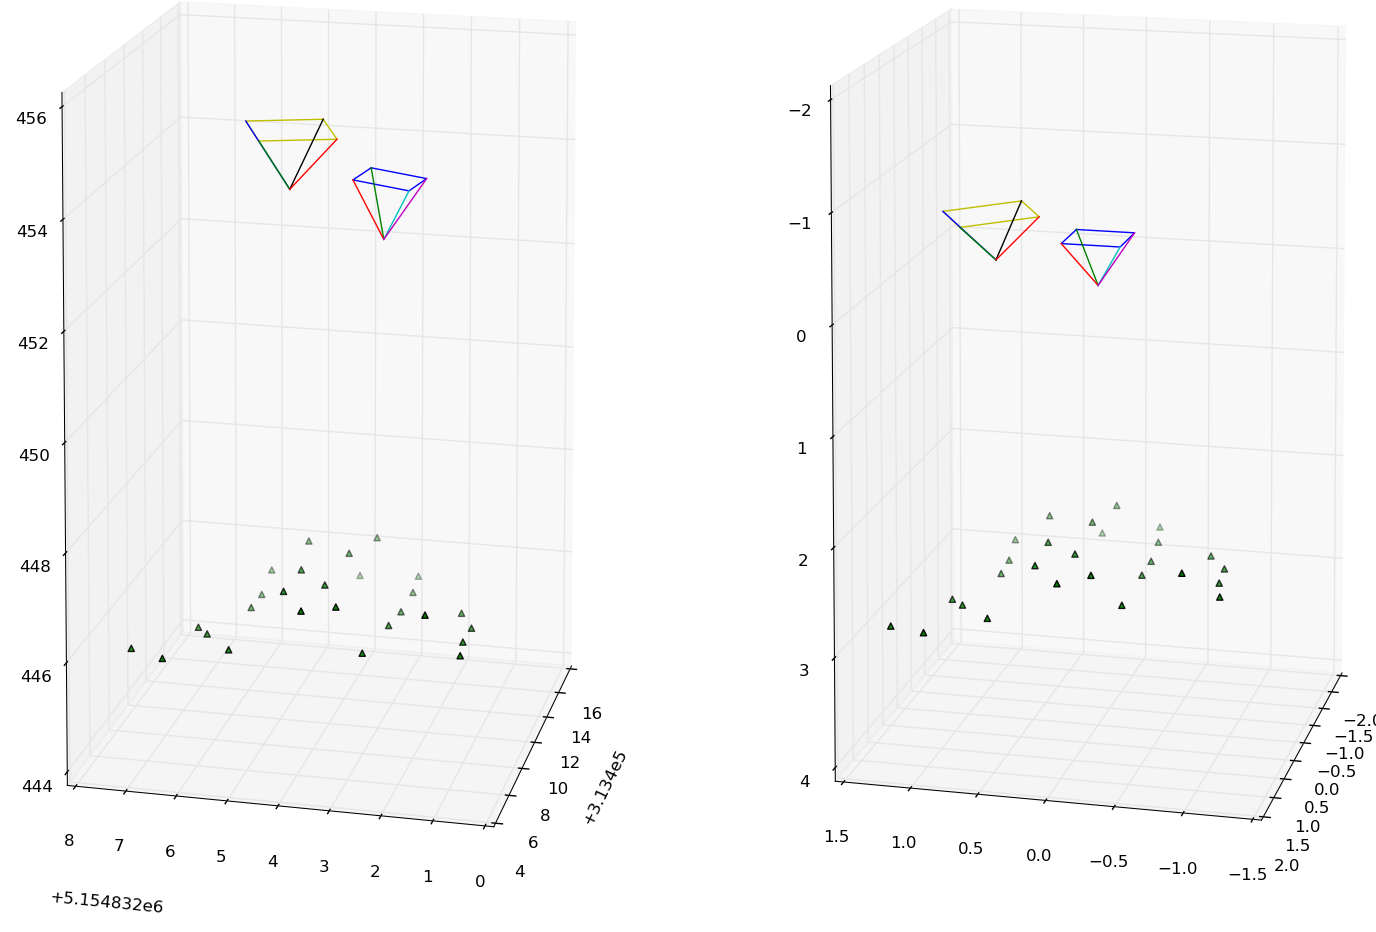
\includegraphics[scale=0.4]{figures/rel_or_576_598.png}
The right plot shows the result of five point algorithm and the left plot shows result of Bingo-F. Note that both 
plots are in different coordinate system, however it is possible to asses it visually. It is clearly visible
that both scenes are very similar.

On the other hand, there exists  few cases, which relative orientation were not successful.  
One of such a cases is relative orientation of photos pair 553 and 591:  
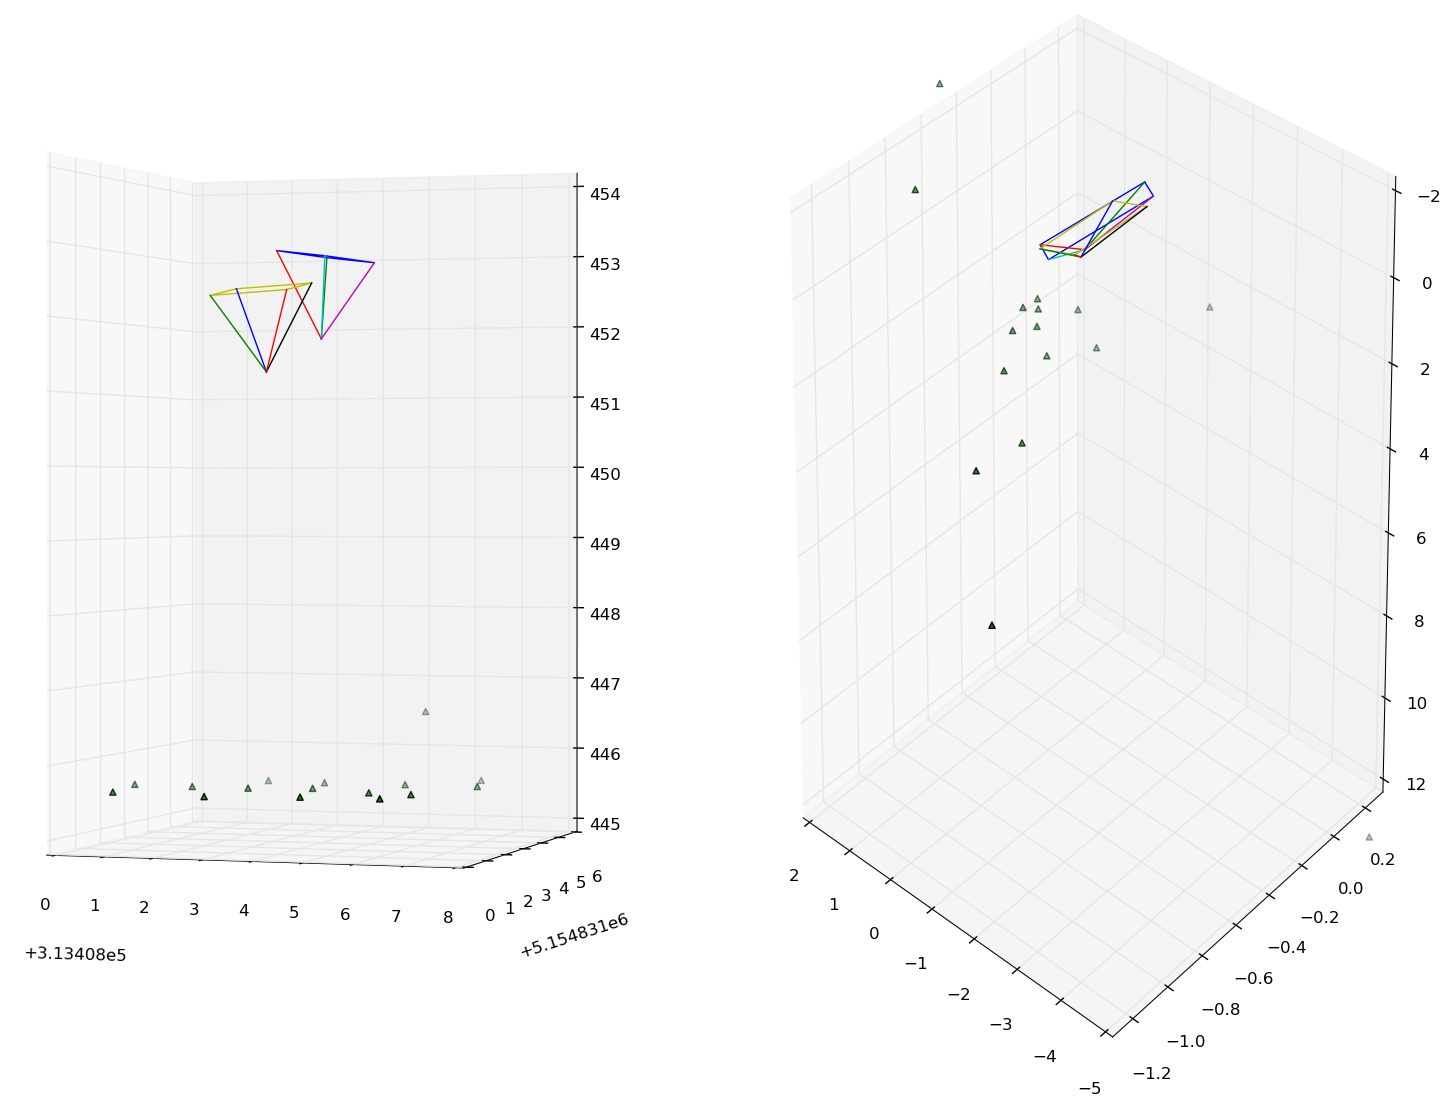
\includegraphics[scale=0.4]{figures/rel_or_553_591.png}
It is clearly visible that result of relative orientation is completely different from the Bingo-F result.
Most important factor, which affects success of the five point algorithm is threshold parameter of RANSAC loop.
The above mentioned relative orientations were computed with RANSAC threshold parameters set to 0.001 mm.
If the threshold parameter is changed in 0.1 mm, the result of relative orientation of pair 553 and 591 improves significantly.
On the other hand another relative orientations go wrong. Therefore with statically set threshold parameter, there is always 
few evidently wrong relative orientations in this scene. Thanks to the configuration of the scene, where lot of photos are 
covering same points, it is  not serious problem, because the point is determined in most relative orientations  with 
much better accuracy, thus it is possible to exclude this outliers. This could be serious problem e. g. if the photos 
of scene would cover long chain where redundancy is much more lower.   
In this case one wrong relative orientation could thread whole result of bba. If error would appear in the middle 
of the chain it would  be propagated up  (TODO reference) one half of the chain which transformation on the wrongly
determined pair, which is apparent from equations in \label{eq:comm_rel}. 
In the test case there are not so many critical pairs, which has to be determined correctly to avoid spoiling the transformation 
of the others dependent pairs. Fortunately the reference pair, which defines common relative system, is very stable and also 
the other  core pairs on which depends lot of other pairs are stable. Probably there is some correlation between number 
of points and stability of five point solution, because as it was already mentioned algorithm of merging searches 
for maximum number of tie points from possible relative orientation, thus another way how to improve stability of the solution 
could be identification of another tie points, which could be done automatically by pattern matching algorithms. 
In the test case there 
are 27 tie points in the reference pair. Which gradually decreases to 6 point in the pair, which is merged as last.

During the merging process all object points computed from different relative orientations, which represents same point are 
transformed into  the common relative system. Then the approximate coordinates by object points are determined as median
of point coordinates from different relative orientations. Median was chosen because it is more robust to the effect of 
big outliers caused by few wrong relative orientations in the set. If there is more than 50 percent of coordinates 
which are close to the correct value and the rest are big outliers (luckily the test case is the case), median gives reasonable results over average,
which is much more sensitive to the effect of the big outliers. 

The next step is helmert transformation from the common relative orientation system into the world coordinate system using available gcps. 
The transformed scene can be compared to the results of Bingo-F adjustment. Average difference of exterior orientation 
of camera is approximately around 0.5 meters with highest outlier in meters. The object points coordinates 
are little bit more accurate with average approximately 20 and highest utliers in 3-1 meters. 
Angles differences are shown in this plot, where there are plotted axes of two camera coordinates systems, which represents 
Bingo-F adjustment angles and the  initial angles. 
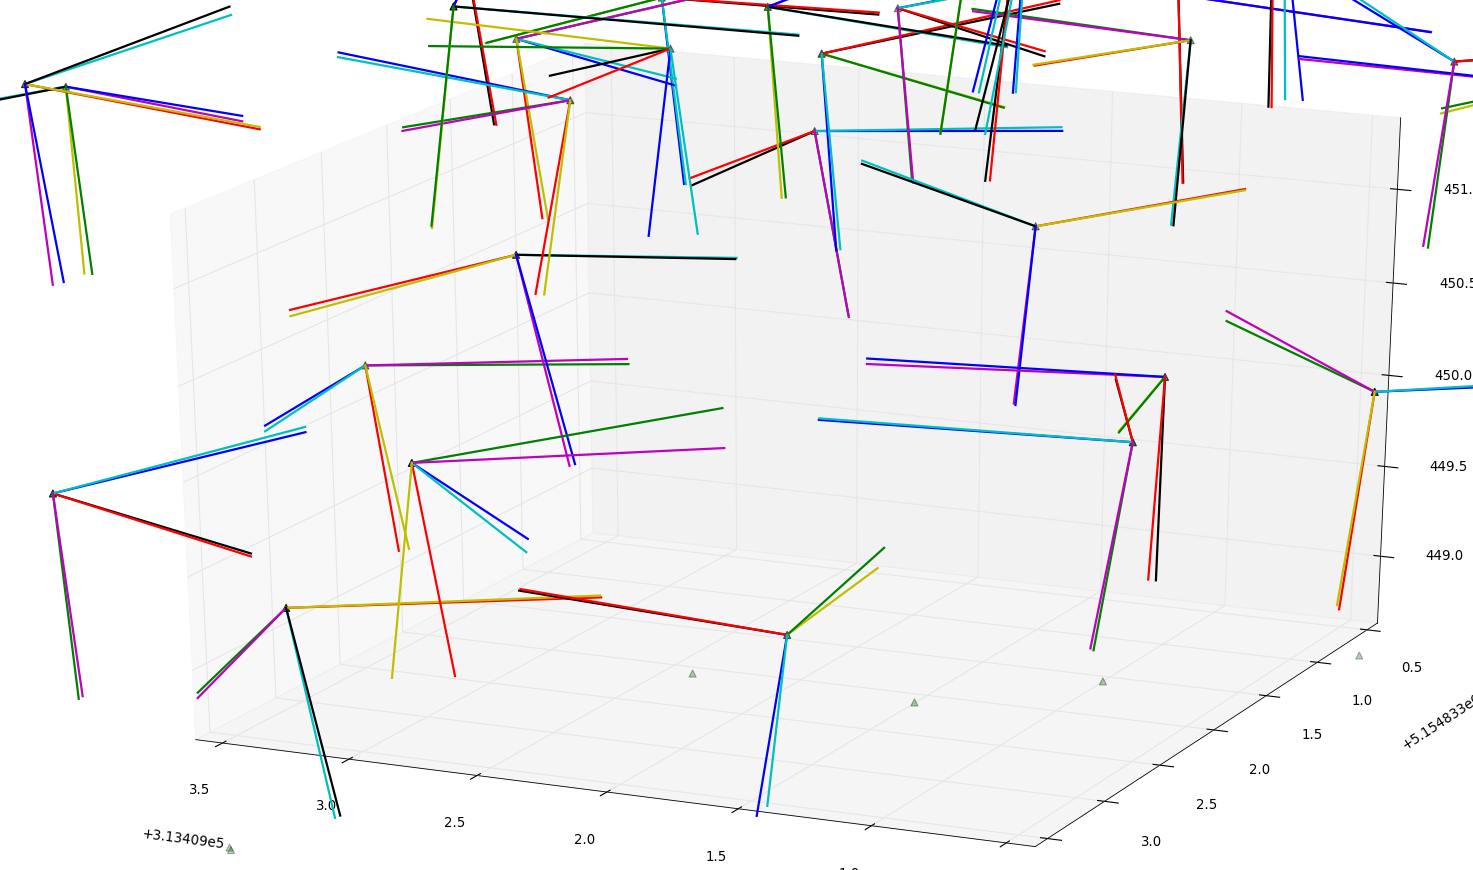
\includegraphics[scale=0.4]{figures/angles_comaprison_relative_orinetaion.png}
It is clear that there are a few orientations, which differs  (tenths of degrees) form the result. 
As a last step bba was applied on these initial values with taking gcp as knowns TODO std in bingo.
Despite the fact that there were few huge outliers in both parameters of cameras and points,
bba after five iteration subsequently refines all scene parameter and reduces all cordinates 
differences into the centimeters and angles into the tenths of degrees. 


This plot again shows differences of cameras coordiantes system, which are no longer visible from this point of view
unlike to the previous plot:
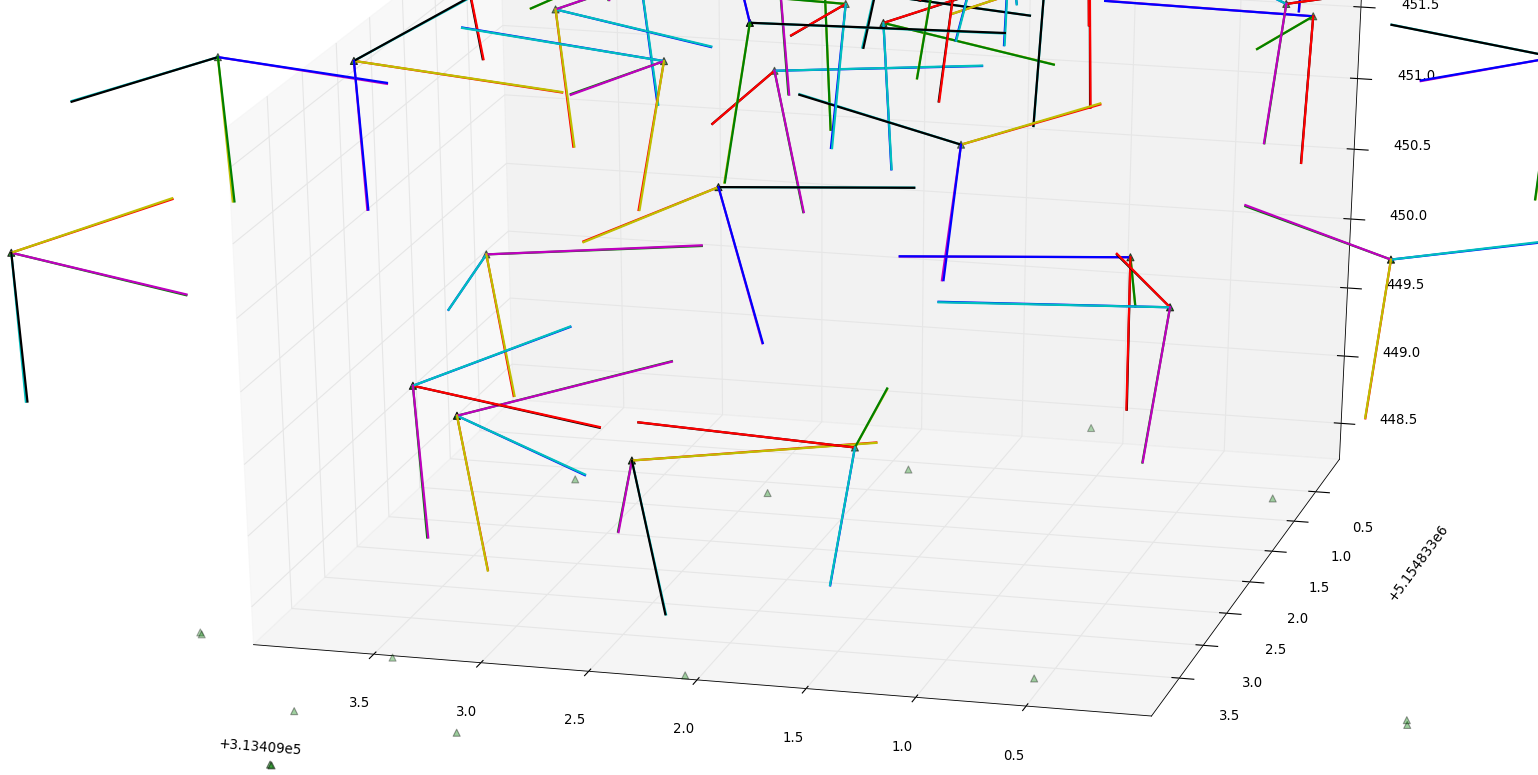
\includegraphics[scale=0.4]{figures/result.png}


\chapter{Future development}

There is lot incredible amount if  work, which can be done in the feature. 
Basically the work which has been done in this thesis, can be considered as prove of concept,
which shows path, which should future implementation of bba in GRASS GIS.


First step, which should be done is basically make whole processing chain workable for users, who 
has good knowledge of photogrammetry or ocomputer vision. Currently  the processing chain was tested 
just on one scene, where it gives some results which makes sense (see previous chapter). However 
author is sure that in other more complicated scenes it would not work successfully because 
the solution is not robust at all.

In order to improve robustness of the processing chain this suggestions should be considered:
\begin{itemize}
\item Relative orientations - there is no check, whether relative orientation accuracy is successful or not. There 
should be implemented some mechanism, which asses quality of relative orientation (probably according to object points reprojection ).
Also it should be examined work of the five point algorithm with RANSAC loop, on scenes with higher number of the tie points, where 
the outliers elimination effect of RANSAC loop should be much stronger.
\item  Merging of relative orientations - currently if there is one wrong relative orientation, with lot of depended relative orientations  
the error gets propagated up during transformer to the common relative coordiante system. Effect of such a inaccurate pair could be 
reduced by performing  temporary bba, which can fix these big inaccuracies. Also the order of relative orientations should not 
be chosen only by number of tie points but also taking into account quality of relative orientation.
\item During final bba, the weights are ignored using identity matrix. Good choice of weights during every bba iteration 
could make the chain significantly robust. Another way how to improve final accuracy of bba is skipping points, which 
standard deviation from adjustment is higher than some results. Worth of exploring are also robust least squares methods,
which uses another probability distribution functions instead of the normal distributu

\item 
\item 
\end{itemize}



\chapter{Future development}




\chapter{Conclusion}

\section{References}
\nobibliography{BP}
\bibliographystyle{plain}
\bibentry{Hartley2004}

\bibentry{wiki:SIFT}

\bibentry{wiki:SURF}

\bibentry{leutenegger2011brisk}

\bibentry{barazzetti2010extraction}

\bibentry{wiki:Eight-point_algorithm}

\bibentry{stewenius2006recent}

\bibentry{bruckner2008experimental}

\bibentry{nister2004efficient}
TODO
\bibentry{pietzsch2001robot}
TODO
\bibentry{pietzsch2004application}

\bibentry{rocchini2012robust}

\bibentry{i.ortho.photo}

\bibentry{neteler2008open}

\bibentry{camera_calibration2013opencv}

\bibentry{zhang2000flexible}

\bibentry{calib_manual2013opencv}

\bibentry{v.rectify}

\bibentry{brown1966distortion}

\bibentry{bingo2013gip}

\section{Appendix}
\subsection{Adjustment protocol}
\label{sec:adj_protocol}


\end{document}}
